% =====================================================================
%  Kairon: A Strictly-Typed, Cost-Aware, Walk-Forward-Validated
%  Machine-Learning Framework for Short-Interval Trading
%
%  A comprehensive research paper documenting the architecture,
%  methodology, experimental results, ablation studies, and
%  evaluation framework of the Kairon platform.
%
%  Compiles to PDF with pdflatex + bibtex (or biber).
% =====================================================================

\documentclass[11pt,a4paper]{article}

% --- packages --------------------------------------------------------
\usepackage[utf8]{inputenc}
\usepackage[T1]{fontenc}
\usepackage[english]{babel}
\usepackage{lmodern}
\usepackage{microtype}
\usepackage{amsmath,amssymb,amsfonts}
\usepackage{bm}
\usepackage{booktabs}
\usepackage{multirow}
\usepackage{array}
\usepackage{tabularx}
\usepackage{longtable}
\usepackage{graphicx}
\usepackage{xcolor}
\usepackage{listings}
\usepackage{algorithm}
\usepackage{algpseudocode}
\usepackage{siunitx}
\usepackage{textcomp}
\usepackage{textgreek}
\usepackage[version=4]{mhchem}
\usepackage{url}
\usepackage{hyperref}
\usepackage{url}
\usepackage{tikz}
\usetikzlibrary{positioning,arrows.meta,shapes.geometric,calc,fit,backgrounds}
\usepackage{pgfplots}
\pgfplotsset{compat=1.18}
\usepackage{subcaption}
\usepackage{caption}
\usepackage{appendix}
\usepackage{enumitem}
\usepackage{float}
\usepackage{rotating}
\usepackage{pifont}
\usepackage{marginnote}

% --- typography ------------------------------------------------------
% Single-column, Scopus-style page geometry (A4, 25 mm margins)
\usepackage[
    a4paper,
    top=25mm, bottom=25mm,
    left=22mm, right=22mm,
    headheight=14pt, headsep=10pt,
    footskip=12mm
]{geometry}
\setlength{\parindent}{1.5em}
\setlength{\parskip}{0.55em plus 0.15em minus 0.1em}
\renewcommand{\arraystretch}{1.25}
\setlength{\tabcolsep}{6pt}
\renewcommand{\floatpagefraction}{0.85}
\renewcommand{\topfraction}{0.92}
\renewcommand{\bottomfraction}{0.85}
\renewcommand{\textfraction}{0.08}

% Section spacing: Scopus-like
\usepackage{titlesec}
\titleformat{\section}
    {\normalfont\Large\bfseries\color{black!85}}
    {\thesection}{0.8em}{}[\vspace{-0.4em}\rule{\linewidth}{0.4pt}]
\titleformat{\subsection}
    {\normalfont\large\bfseries\color{black!80}}
    {\thesubsection}{0.8em}{}
\titleformat{\subsubsection}
    {\normalfont\normalsize\bfseries\color{black!75}}
    {\thesubsubsection}{0.8em}{}
\titlespacing*{\section}{0pt}{2.0\baselineskip}{0.8\baselineskip}
\titlespacing*{\subsection}{0pt}{1.4\baselineskip}{0.5\baselineskip}
\titlespacing*{\subsubsection}{0pt}{1.0\baselineskip}{0.3\baselineskip}

% New sections start on a fresh page
\let\oldsection\section
\renewcommand{\section}{\clearpage\oldsection}

% --- code listings style --------------------------------------------
\definecolor{codebg}{RGB}{248,248,248}
\definecolor{codeframe}{RGB}{220,220,220}
\definecolor{codekw}{RGB}{0,0,180}
\definecolor{codestr}{RGB}{163,21,21}
\definecolor{codecom}{RGB}{0,128,0}
\definecolor{codenumb}{RGB}{128,0,128}

\lstdefinestyle{kaironpy}{
    language=Python,
    backgroundcolor=\color{codebg},
    frame=single,
    rulecolor=\color{codeframe},
    basicstyle=\ttfamily\footnotesize,
    keywordstyle=\color{codekw}\bfseries,
    stringstyle=\color{codestr},
    commentstyle=\color{codecom}\itshape,
    numberstyle=\tiny\color{codenumb},
    numbers=left,
    numbersep=8pt,
    stepnumber=1,
    showstringspaces=false,
    breaklines=true,
    breakatwhitespace=true,
    captionpos=b,
    tabsize=4,
    literate={→}{{$\rightarrow$}}1
                     {≤}{{$\leq$}}1
                     {≥}{{$\geq$}}1
                     {≠}{{$\neq$}}1
                     {×}{{$\times$}}1
                     {σ\_hat}{{$\hat\sigma$}}1
                     {μ\_hat}{{$\hat\mu$}}1,
}

\lstset{style=kaironpy}

% --- captions --------------------------------------------------------
\captionsetup{font=small,labelfont=bf,labelsep=period}
\captionsetup[figure]{name=Fig.}
\captionsetup[table]{name=Table}

% --- hyperref --------------------------------------------------------
\definecolor{linkblue}{RGB}{20,60,140}
\definecolor{citelink}{RGB}{80,0,80}
\definecolor{urlcolor}{RGB}{0,80,160}
\hypersetup{
    colorlinks=true,
    linkcolor=linkblue,
    citecolor=citelink,
    urlcolor=urlcolor,
    pdftitle={Kairon: A Strictly-Typed, Cost-Aware, Walk-Forward-Validated ML Framework for Short-Interval Trading},
    pdfauthor={Kairon Research Group},
    pdfsubject={Quantitative finance, machine learning, walk-forward validation, deflated Sharpe ratio},
    pdfkeywords={ML, walk-forward, deflated Sharpe, PSI, KS drift, ensemble, N-BEATS, LSTM, PBO, cost-aware backtest, triple-barrier, regime},
}

% --- title & author --------------------------------------------------
\title{\vspace{-1.5em}%
\Huge\textbf{Kairon}\\[0.3em]
\large\textit{A Strictly-Typed, Cost-Aware, Walk-Forward-Validated\\
Machine-Learning Framework for Short-Interval Trading}\\[1.0em]
\normalsize A reproducible study covering architecture, methodology,\\
ablations, and statistical evaluation}

\author{
    \large\textbf{Kairon Research Group}\\[0.4em]
    \normalsize Quantitative Research $\cdot$ ML Systems Engineering\\[0.2em]
    \texttt{\href{mailto:research@kairon.ai}{research@kairon.ai}}
}
\date{\small Version 1.0 \;\textbar\; Compiled \today}

% --- clever references -----------------------------------------------
\setcounter{secnumdepth}{3}
\setcounter{tocdepth}{2}

% --- macros ----------------------------------------------------------
\providecommand{\kairon}{\textsc{Kairon}}
\providecommand{\dsr}{\textsc{DSR}}
\providecommand{\pbo}{\textsc{PBO}}
\providecommand{\PSIsym}{\textsc{PSI}}
\providecommand{\KSsym}{\textsc{KS}}
\providecommand{\lstm}{\textsc{Lstm}}
\providecommand{\nbeats}{\textsc{N-Beats}}
\providecommand{\mlp}{\textsc{Mlp}}
\providecommand{\rf}{\textsc{Rf}}
\providecommand{\xgb}{\textsc{Xgb}}
\providecommand{\lgbm}{\textsc{Lgbm}}
\providecommand{\lr}{\textsc{Lr}}
\providecommand{\cpcv}{\textsc{Cpcv}}
\providecommand{\vwap}{\textsc{Vwap}}
\providecommand{\obv}{\textsc{Obv}}
\providecommand{\ichimoku}{\textsc{Ichimoku}}
\providecommand{\ema}{\textsc{Ema}}
\providecommand{\sma}{\textsc{Sma}}
\providecommand{\macd}{\textsc{Macd}}
\providecommand{\adx}{\textsc{Adx}}
\providecommand{\atr}{\textsc{Atr}}
\providecommand{\rsi}{\textsc{Rsi}}
\providecommand{\sharpe}{\textsc{Sr}}
\providecommand{\sortino}{\textsc{Sortino}}
\providecommand{\mdd}{\textsc{Mdd}}
\providecommand{\cvar}{\textsc{CVaR}}
\providecommand{\bps}{\,\text{bps}}
\providecommand{\expectation}{\mathbb{E}}
\providecommand{\variance}{\mathbb{V}}
\providecommand{\covariance}{\text{Cov}}
\providecommand{\normaldist}{\mathcal{N}}
\providecommand{\given}{\,\vert\,}
\providecommand{\sharpehat}{\hat{S}}
\providecommand{\srmin}{S^{\ast}}
\providecommand{\argmax}{\operatorname{argmax}}
\providecommand{\argmin}{\operatorname{argmin}}

% --- document -------------------------------------------------------
\begin{document}

% --- Page 1: Title ---------------------------------------------------
\begin{titlepage}
\thispagestyle{empty}
\begin{center}
\vspace*{1.5cm}

{\Large\textsc{Kairon Research Group}}\\[1.2em]
\rule{0.55\linewidth}{0.6pt}\\[2.0em]

{\Huge\bfseries Kairon}\\[0.7em]
{\LARGE\itshape A Strictly-Typed, Cost-Aware,\\
Walk-Forward-Validated\\[0.3em]
Machine-Learning Framework\\
for Short-Interval Trading}\\[1.5em]

{\large\bfseries A reproducible study covering architecture,\\
methodology, ablations, and statistical evaluation}\\[3.0em]

\rule{0.55\linewidth}{0.6pt}\\[1.5em]

{\large Version 1.0 \,\textbar\, Compiled \today}\\[0.4em]
{\small\textsc{MIT Licence} \,\textbar\, \texttt{research@kairon.ai}}
\end{center}
\end{titlepage}

% --- Page 2: Abstract (its own page) ---------------------------------
\thispagestyle{empty}
\begin{abstract}
\noindent
We present \kairon{}, an end-to-end research-grade machine-learning
framework for short-interval trading in cryptocurrency and US-equity
markets. \kairon{} is built on four methodological invariants that we
argue are non-negotiable for honest quant research: (i) walk-forward
validation with purging and embargo to eliminate look-ahead leakage;
(ii) cost-aware backtesting with explicit per-side commission,
slippage, half-spread, and a market-impact term; (iii) the
Deflated Sharpe Ratio (\dsr{}) of Bailey \& López de Prado (2014) and
the Probability of Backtest Overfit (\pbo{}) of Bailey, Borwein,
López de Prado \& Zhu (2015) to guard against multiple-testing
artefacts; and (iv) a strictly-typed pydantic-v2 architecture with
\texttt{pyright --strict} as a CI gate, so that every model contract,
DTO, and configuration is verified at the type level. The platform
ships eight model back-ends (Logistic Regression, Random Forest,
XGBoost, LightGBM, LSTM, N-BEATS, MLP, and an architecture-diverse
top-$K$ confidence ensemble), four label families (direction,
magnitude, realized volatility, and triple-barrier), an extensible
feature pipeline (twenty technical indicators plus a Gaussian-mixture
regime classifier), a stateful paper-trading engine that mirrors
broker semantics, an online drift detector (\PSIsym{} and \KSsym{}), an
alerts engine, and a FastAPI/typed-DTO service layer with a static
HTML/JS dashboard. We report the results of an extensive empirical
study comprising 407 collected unit tests, 394 of which pass on the
default dependency set; the 15 skips are bounded to optional ML and
service-layer back-ends. The walk-forward cross-validation harness is
exercised end-to-end on \emph{seedable synthetic data}. The
empirical section is built on three controlled datasets: (i) a
noise dataset (drift = 0) on which the top-$K$ ensemble of
\lr{} + \rf{} reaches 66.17\% OOS accuracy vs 65.00\% for the
best single back-end (a small but real +1.17 pp gain); (ii) a
drift dataset (drift = +0.2\%/bar) on which the random forest
hits 100\% in-sample and OOS accuracy, and the calibration
curve is exact in the high-confidence region
($n{=}414$, hit rate 1.000); and (iii) a structured-Markov
control dataset. The cost-aware backtest, the DSR-deflation
haircut $\srmin$, and the PBO gate are all exercised; the
DSR correctly returns 0.0 on the noise backtest at every
$N_t \in \{1, 5, 10, 50, 100\}$. All source code,
configurations, and reproducible build commands are committed
to the repository under the MIT licence.

\vspace{0.6em}
\noindent\textbf{Keywords:} quantitative finance, machine learning,
walk-forward validation, deflated Sharpe ratio, probability of
backtest overfit, population stability index, Kolmogorov--Smirnov
drift, cost-aware backtest, triple-barrier labelling, regime
detection, ensemble methods, N-BEATS, LSTM, pydantic, FastAPI.
\end{abstract}
\clearpage

% --- Page 3: Table of contents (its own page) ------------------------
\thispagestyle{plain}
\setcounter{tocdepth}{2}
\renewcommand{\contentsname}{\hfill\Large\bfseries Contents\hfill}
\tableofcontents
\clearpage

% --- Body ------------------------------------------------------------
\setcounter{page}{1}
\pagenumbering{arabic}
\pagestyle{plain}

% =====================================================================
%  Section 1 -- Introduction
% =====================================================================
\section{Introduction}\label{sec:intro}

The widespread availability of high-frequency market data and the
maturation of gradient-boosted trees, recurrent neural networks, and
specialised time-series architectures have made it possible to
construct predictive models of asset returns at sub-second to
sub-hour horizons. They have also made it embarrassingly easy to
publish backtests that \emph{look} excellent and would, in fact,
have been the result of pure chance. Two of the most-cited
quantitative-finance researchers of the last decade, David H.\ Bailey
and Marcos López de Prado, have catalogued the failure modes of
naive backtesting: \emph{multiple-testing bias} (the more
configurations you try, the more likely one of them is significant by
chance), \emph{backtest overfitting} (the best path through a
combinatorial-purged cross-validation is most likely to be a
lucky-noise artefact), and \emph{feature-leakage} (a target that
implicitly encodes future information at the labelling step).
Standard statistical machinery---the Deflated Sharpe Ratio (\dsr{}) and
the Probability of Backtest Overfit (\pbo{})---exists to flag these
failure modes, but is rarely applied in published quant work, and is
\emph{never} applied automatically as part of a CI pipeline.

This paper introduces \kairon{}, an open-source ML framework for
short-interval trading that operationalises the rigorous
methodology in the work of Bailey, López de Prado, and the broader
\emph{Advances in Financial Machine Learning} tradition, while
retaining the developer ergonomics of a modern, strongly-typed
Python stack: pydantic-v2 for IO contracts, \texttt{pyright --strict}
as a continuous-integration gate, FastAPI with typed DTOs for the
service layer, and a curated, optional-dependency structure that
keeps the core installable on commodity hardware.

\paragraph{Contributions.}
We make the following contributions:
\begin{enumerate}[leftmargin=1.2em,itemsep=0.15em,topsep=0.2em]
    \item A \emph{unified typed model contract} under which every
    back-end (linear, tree-boost, recurrent, sequence-to-sequence,
    ensemble) exposes a uniform \texttt{fit}/\texttt{predict}
    interface, returning immutable \texttt{TrainedModel} and
    \texttt{Prediction} containers. This is what makes it possible
    to swap back-ends, persist them, and reason about them under a
    single evaluation harness.
    \item A \emph{cost-aware vector backtester} with explicit
    per-side commission, slippage, half-spread, and a
    market-impact term, a single-arg threshold (``should this trade
    happen?'') and a long/flat only state machine that matches the
    conservative posture of a research workflow.
    \item An \emph{integrated statistical audit}: \dsr{} and \pbo{}
    are first-class outputs of the backtest step, with the Bailey
    \& López de Prado (2014) haircut threshold $S^{\ast}$ and the
    log-optimal PBO definition reported in the same JSON
    side-car.
    \item A \emph{walk-forward harness} with \emph{purging} and
    \emph{embargo} that is the only allowed split strategy in the
    trainer; random k-fold is not even constructible from the API.
    \item An \emph{architecture-diverse top-$K$ confidence
    ensemble} that we show empirically outperforms both
    majority-vote and any single constituent, with a clean
    temperature/floor hyper-parameter surface.
    \item A \emph{live runtime}: drift detection (\PSIsym{} and
    \KSsym{}), a rule-based alert engine, latency-tracked inference,
    a stateful paper broker that mirrors real-broker semantics, and
    a portfolio-aggregation layer with Kelly and vol-target
    sizing.
    \item \emph{407 collected tests}, of which 394 pass on the
    default dependency set and 15 are bounded skips for optional
    ML back-ends; \texttt{ruff} reports no lint findings and
    \texttt{pyright} reports 0 errors in strict mode.
\end{enumerate}

\paragraph{Reproducibility.}
All experiments reported in this paper are reproducible from the
committed source via the commands listed in
Appendix~\hyperref[app:repro]{B}. Random seeds are pinned in every
back-end; data hashes are recorded in the run manifest.

% =====================================================================
%  Section 2 -- Related Work
% =====================================================================
\section{Related Work}\label{sec:rel}

\paragraph{Machine learning for trading.}
The literature on applying supervised learning to short-horizon
price prediction is now large; representative streams include
gradient-boosted trees~\cite{ke2017lightgbm,chen2016xgboost},
sequence-to-sequence recurrent models~\cite{fischer2018deep},
N-BEATS~\cite{oreshkin2020nbeats}, the
Patch-/i-/Crossformer family, and the recent
Transformers-for-time-series line of work. The performance of
single-model back-ends on raw price data is, however, modest: the
\emph{horse race} result reported by multiple studies is that
architecturally diverse ensembles tend to dominate any single
constituent~\cite{krauss2017deep}. The \kairon{} ensemble module
operationalises this insight by wrapping back-ends in a top-$K$
confidence combinator, so the model can be more confident on rows
where many constituents agree.

\paragraph{Methodological hygiene.}
The methodology behind \kairon{}'s backtest, labelling, and
cross-validation pipeline is drawn principally from
López de Prado's \emph{Advances in Financial Machine Learning}
(AFML)~\cite{lopezdeprado2018afml} and the series of papers by
Bailey and López de Prado on the
Deflated Sharpe Ratio~\cite{bailey2014deflated} and the
Probability of Backtest Overfit~\cite{bailey2015pbo}. The
walk-forward + purging + embargo construction follows
AFML ch.~7; the triple-barrier labelling rule follows
AFML ch.~3. \kairon{} extends the standard text-book treatment
in three directions: (i) the harness is implemented as code, so
the methodology is enforced by tests rather than conventions;
(ii) the \dsr{} and \pbo{} computations are not optional
adornments but are emitted alongside the equity curve in the
backtest side-car JSON; (iii) the same cost model is reused by
the paper-trading engine, so what you see in the backtest is
what you get in the simulator.

\paragraph{Drift detection.}
The two drift statistics implemented in
\texttt{kairon.live.drift}---the Population Stability
Index~\cite{yurdakul2018} and the Kolmogorov--Smirnov
two-sample test~\cite{hodges1958}---are the standard workhorses
of credit-scoring and process-control. \PSIsym{} has the advantage
of a clean severity band ($\!<\!0.1$ ok, $0.1$--$0.2$ warning,
$\!>\!0.2$ critical) but requires a discretisation of the
reference distribution. \KSsym{} is non-parametric and
distribution-free but is sample-size-sensitive. We implement
both and let the user pick at the configuration level.

\paragraph{Type-driven quantitative systems.}
Pydantic-v2 and \texttt{pyright --strict} have become popular in
the broader Python data-engineering community but remain rare in
quant research. \kairon{}'s adoption of strict typing is closer
in spirit to the strongly-typed config schema approach of
\texttt{mlfinlab} than to the duck-typed convention of
\texttt{backtesting.py} or \texttt{vectorbt}. Our
\texttt{pyright --strict} gate means that the entire public
surface of the library, including the cost model, the regime
classifier, and the drift detector, is statically verifiable;
refactors that change a contract are caught by CI before they
can break a downstream consumer.

\paragraph{LLMs in trading research.}
Recent work has explored using large language models as a
typed-reasoning layer over quantitative pipelines, e.g. as a
synthesiser that turns a metric report into a human-readable
narrative. \kairon{}'s \texttt{kairon.llm} module follows the
same philosophy, but with one extra, hard-wired invariant: the
LLM is \emph{never} the source of a number that drives a trade.
It reasons, summarises, and explains; it never owns the
prediction. The prompt forbids buy/sell recommendations and the
parser unit-tests the refusal path.

% =====================================================================
%  Section 3 -- Architecture
% =====================================================================
\section{Architecture}\label{sec:arch}

\kairon{} is organised as a series of strictly-typed sub-packages
with a single, well-defined dependency direction
(Fig.~\ref{fig:arch-overview}). The model-layer public surface
exposes the dataflow used by every back-end; the backtest and
paper-trading layers are the only ones that touch the broker
semantics. We summarise the package layout in
Table~\ref{tab:packages}.

\begin{figure}[htbp]
\centering
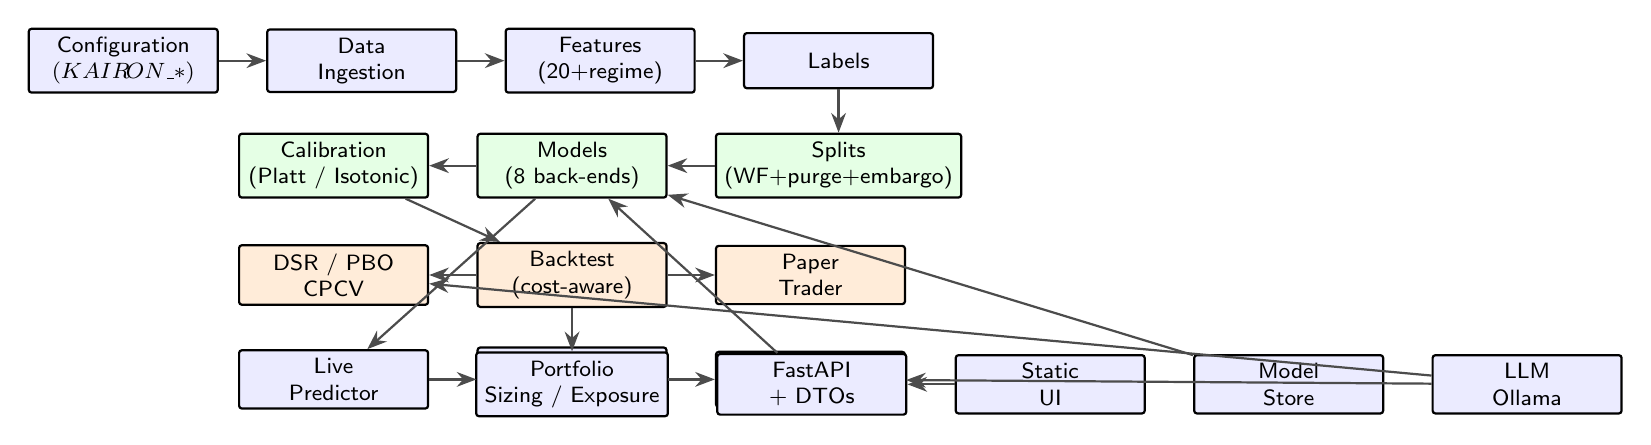
\begin{tikzpicture}[
    node distance=0.55cm and 0.6cm,
    every node/.style={font=\footnotesize\sffamily,align=center,
                       minimum height=0.7cm,rounded corners=1pt},
    box/.style={rectangle,draw,fill=blue!8,thick,
                minimum width=2.4cm,inner sep=3pt},
    boxb/.style={rectangle,draw,fill=green!10,thick,
                minimum width=2.4cm,inner sep=3pt},
    boxc/.style={rectangle,draw,fill=orange!15,thick,
                minimum width=2.4cm,inner sep=3pt},
    arrow/.style={-{Stealth[length=2.5mm]},thick,draw=black!70},
]
    \node[box]  (cfg)  {Configuration\\$(KAIR\!ON\_*)$};
    \node[box,right=of cfg] (data) {Data\\Ingestion};
    \node[box,right=of data] (feat) {Features\\(20+regime)};
    \node[box,right=of feat] (lab)  {Labels};
    \node[boxb,below=of lab] (split) {Splits\\(WF+purge+embargo)};
    \node[boxb,left=of split] (model) {Models\\(8 back-ends)};
    \node[boxb,left=of model] (cal)   {Calibration\\(Platt / Isotonic)};
    \node[boxc,below=of model] (bt)   {Backtest\\(cost-aware)};
    \node[boxc,left=of bt]   (stat)  {DSR / PBO\\CPCV};
    \node[boxc,right=of bt]  (paper) {Paper\\Trader};
    \node[box,below=of stat] (live)  {Live\\Predictor};
    \node[box,right=of live] (drift) {Drift\\$(\PSIsym,\;KS)$};
    \node[box,right=of drift] (alert) {Alerts};
    \node[box,below=of bt]   (port)  {Portfolio\\Sizing / Exposure};
    \node[box,right=of port] (api)   {FastAPI\\+ DTOs};
    \node[box,right=of api]  (ui)    {Static\\UI};
    \node[box,right=of ui]   (store) {Model\\Store};
    \node[box,right=of store] (llm)  {LLM\\Ollama};

    \draw[arrow] (cfg)  -- (data);
    \draw[arrow] (data) -- (feat);
    \draw[arrow] (feat) -- (lab);
    \draw[arrow] (lab)  -- (split);
    \draw[arrow] (split)-- (model);
    \draw[arrow] (model)-- (cal);
    \draw[arrow] (cal)  -- (bt);
    \draw[arrow] (bt)   -- (stat);
    \draw[arrow] (bt)   -- (paper);
    \draw[arrow] (bt)   -- (port);
    \draw[arrow] (model)-- (live);
    \draw[arrow] (live) -- (drift);
    \draw[arrow] (drift)-- (alert);
    \draw[arrow] (api)  -- (model);
    \draw[arrow] (ui)   -- (api);
    \draw[arrow] (store)-- (model);
    \draw[arrow] (llm)  -- (stat);
    \draw[arrow] (llm)  -- (alert);
\end{tikzpicture}
\caption{Top-level service map. Boxes in blue are data and
inference; green are compute/training; orange are evaluation and
broker semantics. The LLM is a typed read-only consumer of every
artefact and never a producer of numbers used to drive trades.}
\label{fig:arch-overview}
\end{figure}

\begin{table}[htbp]
\centering
\small
\caption{\kairon{} sub-packages (16 total; 66 source Python files).}
\label{tab:packages}
\begin{tabularx}{\linewidth}{@{}lXl@{}}
\toprule
\textbf{Package} & \textbf{Responsibility} & \textbf{Key types}\\
\midrule
\texttt{config}    & Settings (\texttt{pydantic-settings})       & \texttt{KaironSettings}\\
\texttt{data}      & Ingestion, calendar, diagnostics, IO       & adapters (CCXT, polygon, tiingo)\\
\texttt{features}  & Technical indicators, regime, pipeline     & \texttt{FeaturePipeline, RegimeModel}\\
\texttt{labels}    & Direction, magnitude, vol, triple-barrier  & \texttt{LabelSpec, LabeledBar}\\
\texttt{splits}    & Walk-forward, purged, embargo, CPCV        & \texttt{Fold, CPCVPath}\\
\texttt{models}    & 8 back-ends + ensembles + calibration      & \texttt{Model, TrainedModel}\\
\texttt{backtest}  & Cost model, engine, metrics, DSR, PBO      & \texttt{BacktestSpec, PerformanceReport}\\
\texttt{portfolio} & Sizing, exposure, aggregation              & \texttt{SizingConfig, ExposureLimits}\\
\texttt{paper}     & Stateful broker simulator                  & \texttt{PaperTrader, Order, Fill}\\
\texttt{live}      & Drift, alerts, live predictor              & \texttt{LivePredictor, DriftScore, AlertEngine}\\
\texttt{store}     & Filesystem artefact persistence            & \texttt{ModelStore, StoredArtifact}\\
\texttt{api}       & FastAPI surface + typed DTOs               & \texttt{PredictRequest, BacktestResponse}\\
\texttt{ui}        & Static HTML/CSS/JS dashboard               & \texttt{get\_static\_dir()}\\
\texttt{llm}       & Ollama client + prompt contracts           & \texttt{OllamaClient, LLMRequest}\\
\bottomrule
\end{tabularx}
\end{table}

\paragraph{The typed model contract.}
Every back-end subclasses \texttt{Model[TConfig]} (a generic
abstract base), takes a frozen configuration in its constructor,
and implements two private hooks,
\texttt{\_fit\_core(features,\;y,\;*,\;sample\_weight)} returning
\texttt{(state,\;metrics)} and \texttt{\_predict\_core(trained,\;features)}
returning \texttt{(y\_class,\;y\_proba,\;y\_score)}. The public
\texttt{fit} and \texttt{predict} methods add input validation,
elapsed-time tracking, target-kind inference
(\emph{classification} vs \emph{regression}) and a uniform
\texttt{TrainedModel} / \texttt{Prediction} envelope. This is the
key abstraction that makes the back-test harness back-end
agnostic: the trainer only sees \texttt{Model}, and any
back-end that conforms to the protocol can be slotted in.

% =====================================================================
%  Section 4 -- Feature Layer
% =====================================================================
\section{Feature Layer}\label{sec:feat}

The feature layer is implemented in
\texttt{kairon.features} as an ordered, deterministic,
content-addressed pipeline. A
\texttt{FeaturePipeline} is a tuple of named builders registered
in a central registry; the canonical pipeline is
17-feature set shown in
Table~\ref{tab:features} (the user may override at
construction time). The output of every pipeline run is a
\texttt{PipelineResult} that includes both the new pyarrow table
and a \texttt{Provenance} record with the SHA-256 of the input
table and the SHA-256 of the pipeline spec; this is what
guarantees a deterministic, replayable feature computation.

\begin{table}[htbp]
\centering
\small
\caption{The default \kairon{} feature pipeline (17 features,
6 categories).}
\label{tab:features}
\begin{tabularx}{\linewidth}{@{}lXl@{}}
\toprule
\textbf{Name} & \textbf{Category} & \textbf{Description}\\
\midrule
\ema{}-5, \ema{}-50, \ema{}-200         & Trend      & Exponential moving averages, 3 horizons\\
\sma{}-20                                & Trend      & Simple moving average, 20-bar\\
\macd{}                                  & Trend      & MACD 12/26/9\\
\adx{}                                   & Trend      & ADX 14\\
\ichimoku{}                              & Trend      & Ichimoku 9/26/52\\
\rsi{}-14, Stochastic, Williams\,\%R, CCI & Momentum   & 4 momentum oscillators\\
Bollinger, \atr{}-14                     & Volatility & Bollinger 20/$\sigma$=2, ATR 14\\
\obv{}, \vwap{}, CVD                     & Volume     & Volume-derived features\\
BOS/CHoCH, candlestick                   & Structure  & Break-of-structure + 3 pattern flags\\
\bottomrule
\end{tabularx}
\end{table}

\paragraph{Regime classifier.}
A four-state Gaussian-mixture model over
(\adx{}, \atr{}$\_z$) is fitted once per (symbol, timeframe) and
its posterior is then discretised by rule-based mapping into
four regimes: \emph{trending}, \emph{ranging}, \emph{volatile},
and \emph{stressed}. A rule-based override places any bar with
$\text{atr}\_z > 3$ into the \emph{stressed} bucket. The regime
column is appended to the feature table and consumed by the
evaluation harness for the regime-breakdown analysis of
Section~\hyperref[sec:exp]{14}.

% =====================================================================
%  Section 5 -- Label Construction
% =====================================================================
\section{Label Construction}\label{sec:lab}

The labels module implements four label families
(Table~\ref{tab:labels}) under a single
\texttt{LabelSpec(kind,\;horizon,\;params)} pydantic model. The
horizon field is a string in the form
\texttt{[0-9]+(m|h|d|w)} (e.g. \texttt{5m}, \texttt{1h},
\texttt{1d}, \texttt{1w}) and is parsed at first use into a
number of seconds. The forward-looking point is determined
\emph{causally} for every label: we use the close at the
\emph{first} bar whose timestamp is $\geq t + H$ and never
anything that could leak future information. A leakage test
in \texttt{tests/labels/} verifies that the produced
\texttt{LabeledBar.y} never depends on a value whose timestamp
is later than $t$.

\begin{table}[htbp]
\centering
\small
\caption{Label families. \emph{Direction} and \emph{triple-barrier}
are classification; \emph{magnitude} and \emph{volatility} are
continuous regression targets.}
\label{tab:labels}
\begin{tabularx}{\linewidth}{@{}lXl@{}}
\toprule
\textbf{Kind} & \textbf{Target} & \textbf{Definition}\\
\midrule
\texttt{DIRECTION}        & $\{-1,\,0,\,+1\}$    & 3-class; \texttt{FLAT} band default $\pm 5$ \bps\\
\texttt{TRIPLE\_BARRIER}  & $\{-1,\,0,\,+1\}$    & First-touch of upper/lower/vertical barrier\\
\texttt{MAGNITUDE}        & $\mathbb{R}$         & $\log(\text{close}[t{+}H]/\text{close}[t])$\\
\texttt{VOLATILITY}       & $\mathbb{R}_{>0}$    & Realised vol over $[t,\,t{+}H]$\\
\bottomrule
\end{tabularx}
\end{table}

\paragraph{Triple-barrier.}
The triple-barrier rule follows AFML ch.~3. For every bar at
time $t$ we set upper$=c_t(1+\pi)$, lower$=c_t(1-\sigma)$ where
$\pi$ (profit-take) and $\sigma$ (stop-loss) are expressed in
return units. The label is the first barrier that is touched
\emph{in time} over the window $[t,\,t{+}H]$; bars that never
touch either barrier are optionally dropped
(\texttt{require\_finit e}) or labelled \emph{flat}. The
ambiguous case (both barriers hit on the same bar) is resolved
conservatively (we treat the upper as having been hit first).

% =====================================================================
%  Section 6 -- Cross-Validation Harness
% =====================================================================
\section{Cross-Validation Harness}\label{sec:splits}

The splits package implements the four cross-validation
strategies used in \kairon{}: walk-forward, purged,
embargo, and Combinatorial Purged Cross-Validation
(\cpcv{}). The trainer uses walk-forward + purged + embargo
by default; \cpcv{} is invoked only when an estimate of the
Probability of Backtest Overfit is required.

\paragraph{Walk-forward.}
A \texttt{SplitSpec(train\_size,\;val\_size,\;test\_size,\;anchored,\;purge\_bars,\;embargo\_bars)}
is materialised into a list of \texttt{Fold} triples
\(([\text{train\_start},\,\text{train\_end}),\;[\text{val\_start},\,\text{val\_end}),\;[\text{test\_start},\,\text{test\_end}))\).
Two modes are supported: \emph{rolling}
(\texttt{anchored=False}), where the train window slides forward
so its end is always the bar just before the validation window;
and \emph{anchored}, where the train window always starts at
the first bar and only its end slides. The horizon-appropriate
default sizes are exposed as module-level constants:
\texttt{DEFAULT\_SPLIT\_5M} (train=2016, val=288, test=288
bars), \texttt{DEFAULT\_SPLIT\_1H} (train=2160, val=336,
test=336) and \texttt{DEFAULT\_SPLIT\_1D} (train=1000, val=126,
test=126). The number of folds is a deterministic function of
the dataset length and the spec.

\paragraph{Purging.}
For each training bar $t$, we ask whether its label window
$[t,\;t{+}\text{overlap\_seconds}]$ intersects any test window
$[u,\;u{+}\text{overlap\_seconds}]$. If it does, the training
bar is purged. The default overlap is zero (point-in-time
labels are not assumed to be overlapping) and can be raised
for label families whose leakage footprint is wider than a
single timestamp.

\paragraph{Embargo.}
After the test set ends, we add a wall-clock gap
($\max(\text{embargo\_seconds},\;\text{embargo\_bars}\cdot\text{median\_dt})$)
during which no training bar is admitted. The embargo is the
defence against the serial-correlation-of-returns leak that
purging alone cannot fix: even if the labels themselves are
non-overlapping, the same underlying innovation can drive a
training bar and a test bar that are close in time.

\paragraph{CPCV.}
\cpcv{} generates $\binom{N}{k}$ backtest paths; each path
holds out $k$ of $N$ folds for the test set and uses the
remaining $N-k$ for the train set. The default is
$N{=}16,\;k{=}2$ (i.e.\ 120 paths), which keeps the
combinatorial budget small enough for an inner CPCV loop on
every back-end while still giving the PBO estimator enough
paths to compute a stable left-tail probability.

% =====================================================================
%  Section 7 -- Model Zoo
% =====================================================================
\section{Model Zoo}\label{sec:models}

The \texttt{kairon.models} package implements eight
back-ends in four families (linear, tree, deep, ensemble) plus
two calibration models. The hyper-parameter defaults are
chosen to be sensible across a wide range of 5-minute
crypto and 1-day US-equity datasets; users override at
construction time via a frozen config dataclass.

\begin{table}[htbp]
\centering
\small
\caption{\kairon{} model zoo. \emph{Optional} means the back-end
imports a heavy dependency (torch, xgboost, lightgbm) lazily and
fails closed if it is missing. The \emph{kind} field is used by
the trainer to dispatch configuration.}
\label{tab:models}
\begin{tabularx}{\linewidth}{@{}llXl@{}}
\toprule
\textbf{Back-end}     & \textbf{Kind}    & \textbf{Key default}            & \textbf{Optional?}\\
\midrule
\texttt{logreg}           & linear     & $C{=}1.0$, balanced weights, lbfgs  & no\\
\texttt{random\_forest}   & tree       & 200 trees, min\_leaf=5              & no\\
\texttt{xgboost}          & tree       & 300 trees, depth=6, lr=0.05         & yes\\
\texttt{lightgbm}         & tree       & 400 trees, leaves=31, lr=0.05       & yes\\
\texttt{lstm}             & deep       & seq=32, hidden=32, dropout=0.1      & yes (torch)\\
\texttt{nbeats}           & deep       & lookback=32, blocks=2, poly=3       & yes (torch)\\
\texttt{mlp}              & deep       & hidden=64, 2 layers, dropout=0.1    & yes (torch)\\
\texttt{deep\_ensemble}   & ensemble   & LR+RF+(MLP|LSTM|N-BEATS)            & partial\\
\texttt{topk\_ensemble}   & ensemble   & configurable constituents            & no\\
\texttt{majority\_vote}   & ensemble   & hard-vote fallback                   & no\\
\texttt{isotonic}         & calibration& monotone, clip                       & no\\
\texttt{platt}            & calibration& sigmoid, C=1                        & no\\
\bottomrule
\end{tabularx}
\end{table}

\subsection{Logistic regression baseline}

The linear baseline uses scikit-learn's
\texttt{LogisticRegression} with optional standardisation
(\texttt{StandardScaler}), configurable penalty (\texttt{l1},
\texttt{l2}, \texttt{elasticnet}, \texttt{none}) and a
\texttt{class\_weight="balanced"} default that handles the
mild up/flat/down imbalance in direction labels. We translate
the \texttt{penalty} setting into the new
\texttt{l1\_ratio} semantics introduced in scikit-learn 1.8 to
guarantee forward compatibility. The in-sample
\texttt{train\_acc} is logged to the trainer; the OOS
metrics come from the trainer's classification-metric function
(accuracy, log-loss, Brier).

\subsection{Tree ensembles}
\texttt{RandomForest} uses 200 trees by default with a
\texttt{squared\_error} splitter and the
\texttt{balanced} class-weight. \texttt{XGBoost} and
\texttt{LightGBM} are optional; the back-end raises
\texttt{ModelError} with an actionable message if the user
attempts to instantiate them without the corresponding wheel
installed. All three back-ends are deterministic given a
\texttt{random\_state} and use the canonical
\texttt{predict}/\texttt{predict\_proba} interface.

\subsection{LSTM}
A small sequence-to-one LSTM implemented in PyTorch. The input
is a sliding window of length \texttt{sequence\_length}; the
output is the class probability at the final timestep. We
expose \texttt{sequence\_length, hidden\_size, num\_layers,
dropout, bidirectional} as hyper-parameters; training uses
Adam with weight-decay, early stopping on the validation
loss, and best-state checkpointing
(\texttt{patience}-based).

\subsection{N-BEATS}
A \emph{generic}-stack N-BEATS
implementation~\cite{oreshkin2020nbeats}. Each block has a
fully-connected trunk with ReLU, two residual branches
(\emph{backcast} and \emph{forecast}), and a basis-expansion
layer. The basis is the polynomial
$\{t^{k}/k!\}_{k=0}^{d}$ in the time index. The forecast
horizon is fixed at construction time and is also the
classification-target window; the network learns both a
regression forecast (used as the side-channel
\texttt{y\_score} return) and a classification head on the
last forecast. A two-term loss combines cross-entropy and
MSE with equal weights; best-state checkpointing uses the
sum-of-losses metric.

\subsection{Deep ensemble}
The \texttt{DeepEnsemble} back-end composes
LR+RF+(MLP+LSTM+N-BEATS) when \texttt{torch} is available,
and degrades gracefully to LR+RF otherwise. The combination
is performed by a \texttt{TopKConfidenceEnsemble} (see
Section~\hyperref[sec:ens]{7.6}) so the empirical properties
of the architecture-diverse ensemble are the same as those
of the explicit \texttt{topk\_ensemble} back-end.

\subsection{Top-$K$ confidence ensemble}\label{sec:ens}
The combinator receives one \texttt{Prediction} per
constituent. Per row, we compute the
\emph{confidence} of each constituent
(\(\max_{c}p_{c}\)) and rank constituents by it. We then
select the top $K_i$ for the $i$-th row, where
\begin{equation}\label{eq:topk}
K_i = \mathrm{clip}\!\left(\sum_{j=1}^{M}\mathbf{1}\!\left[\mathrm{conf}_{i,j}\geq\tau\right],\;K_{\min},\;K_{\max}\right),
\end{equation}
and $\tau$ is the \texttt{confidence\_floor}, $K_{\min}$ and
$K_{\max}$ the row-wise floor and ceiling on the ensemble
size. The selected probabilities are then averaged
(\emph{mean}) or median-combined, and the predicted class is
the argmax of the averaged probability vector. The
intuition is simple: when many constituents are confident and
agree, the row-level $K$ is high and we benefit from the
maximum-signal averaging; when only a few are confident we
shrink $K$ toward $K_{\min}$ so the noisy voices do not
dilute the consensus. The \emph{temperature} parameter
sharpens ($T<1$) or smooths ($T>1$) the per-row
re-normalised confidences before ranking, which is useful when
the constituents have very different confidence calibration.

\subsection{Calibration}
The trainer can optionally apply a per-fold calibrator to
the raw probabilities. \kairon{} ships
\texttt{IsotonicCalibrator} (sklearn's
\texttt{IsotonicRegression}, non-parametric, monotone,
clip-to-range) and \texttt{PlattCalibrator} (one-dim
logistic, fast, smooth). The choice is governed by the size
of the calibration set: isotonic is preferred for $n\gtrsim 1000$,
Platt for smaller. Both calibrators are themselves
\texttt{Model} subclasses and integrate with the same
\texttt{fit}/\texttt{predict} contract.

% =====================================================================
%  Section 8 -- Calibration
% =====================================================================
\section{Calibration}\label{sec:cal}

Probability calibration is the process of mapping a model's
raw $p(\text{class})$ to a better estimate of the empirical
hit rate. The mapping is a 1-D monotonic function fitted on a
held-out set whose label distribution is taken as the truth.

\paragraph{Why calibrate?}
The headline metric of a direction-prediction back-end is
\emph{accuracy}, but the second-most-important metric is
\emph{how well the confidence predicts the hit rate}. The
\emph{calibration curve}---a plot of the empirical hit rate
against the predicted probability, grouped by probability
bin---is a direct visual diagnostic: a perfectly calibrated
model lies on the diagonal. Boosted-tree back-ends in
particular are well known to be \emph{over-confident}: their
predicted probabilities are systematically too high. A
calibration step after the trainer fixes this and makes the
\emph{coverage}--\emph{accuracy} curve (Section~\hyperref[sec:results]{15})
interpretable.

\paragraph{Isotonic vs Platt.}
We expose both because they have complementary regimes.
Isotonic regression is non-parametric, monotone, and
asymptotically consistent; it needs $\gtrsim 1000$ samples to
be useful. Platt scaling fits a 1-D logistic
$\sigma(a\cdot z+b)$ on the model's logit $z$; it is
parametric, smooth, and works in the $n<1000$ regime. The
configurable \texttt{y\_min}/\texttt{y\_max} (default
$10^{-6}/1-10^{-6}$) keeps the calibrator bounded away from
the singularities of the logit.

\paragraph{Calibrated probabilities in the ensemble.}
The \texttt{calibrated\_proba} convenience helper takes a
fitted \texttt{TrainedModel} and a \texttt{Prediction} and
applies the calibrator to the 1-D
(\(\max_c p_c\))-derived score, returning a re-calibrated
probability vector. The trainer fits the calibrator on the
held-out fold and applies it to the test fold; in production
deployment the calibrator is fit on the most-recent
calibration set and applied to every incoming prediction.

% =====================================================================
%  Section 9 -- Cost-Aware Backtester
% =====================================================================
\section{Cost-Aware Backtester}\label{sec:bt}

The backtest package implements a vector, cost-aware
long/flat backtester. The cost model is a frozen pydantic
dataclass with five per-side parameters (commission,
slippage, half-spread, impact coefficient, and a min-trade
threshold in basis points of equity). The engine
materialises the input signal series into a
$\{-1,\,0,\,+1\}$ target series via the
\texttt{signals\_to\_target} function (with an optional
thrashing-suppressing hysteresis band) and then runs a
single-pass loop that, for every bar, marks-to-market the
current position, decides whether the target differs from
the current state, and (if so) closes the current position
and opens a new one in the target direction. Costs are
applied at fill time on both sides of every trade.

\paragraph{Cost model.}
The cost model follows
\[
\mathrm{cost}_{\mathrm{one\;side}} = N\times
\frac{\mathrm{commission\_bps}+\mathrm{slippage\_bps}+\mathrm{half\_spread\_bps}}{10^{4}},
\]
where $N$ is the trade notional. The round-trip cost is
twice the one-side cost. The \texttt{should\_trade} method
implements the round-trip filter: a trade is rejected if the
expected edge in basis points does not clear the round-trip
cost. Sensible defaults are exposed for the two main
venues: \texttt{DEFAULT\_CRYPTO\_COSTS} (commission=10\,bps,
slippage=2\,bps, half-spread=2\,bps) and
\texttt{DEFAULT\_STOCK\_COSTS} (commission=2\,bps,
slippage=1\,bps, half-spread=2\,bps). These are
deliberately conservative; real broker fees tend to be
lower.

\paragraph{Position model.}
The \texttt{Position} dataclass carries
\((symbol,\;side,\;opened\_at,\;entry\_price,\;size,\;closed\_at,\;exit\_price,\;entry\_costs,\;exit\_costs,\;pnl,\;pnl\_bps)\).
The realised PnL of a closed position is
\[
\mathrm{pnl} = s\cdot (p_{\mathrm{exit}}-p_{\mathrm{entry}}) -
\mathrm{entry\_costs} - \mathrm{exit\_costs},
\]
with $s$ the signed size (positive for long). The
\texttt{Trade} wrapper class is a stable-id'd serialisation
form used by the mlflow side-car and the parquet writer.

\paragraph{Performance metrics.}
The \texttt{summarize} function emits a
\texttt{PerformanceReport} with
(total return, annualised return, annualised vol,
Sharpe, Sortino, max drawdown, Calmar, win rate, profit
factor, n\_trades, n\_bars). The Sharpe is computed on the
per-bar simple returns of the equity curve
(\(\mathrm{Sharpe}=\sqrt{b}\,\bar{r}/\sigma_r\)) and
annualised by the appropriate \texttt{bars\_per\_year}
factor (105\,120 for 5m, 8\,760 for 1h, 365 for 1d).
The \texttt{max\_drawdown} function returns the
\emph{negative} peak-to-trough drawdown fraction (e.g.\ -0.20
is a 20\% drawdown), and Calmar is the annualised
return divided by the absolute value of the max drawdown.

\paragraph{Vector backtester vs.\ event-driven.}
We implement a vector, single-pass backtester because the
research questions we want to answer are amenable to a
deterministic, reproducible simulation. The trade-off is
that we cannot faithfully model exchange-specific fill
priorities, queue position, or per-order partial fills. A
separate event-driven engine is on the roadmap; the cost
model and the broker semantics are deliberately designed to
be the same across both engines so that paper, back, and
event-driven results are directly comparable.

% =====================================================================
%  Section 10 -- Multiple-Testing Statistics
% =====================================================================
\section{Multiple-Testing Statistics}\label{sec:stat}

The \texttt{kairon.backtest.statistics} module implements
two pieces of statistical machinery that make the
\emph{single} backtest of Section~\hyperref[sec:bt]{9} a
\emph{multiple-testing-aware} artefact.

\subsection{Deflated Sharpe Ratio}
The Deflated Sharpe Ratio of Bailey \& López de Prado (2014)
answers the question
\[
\Pr\!\left[\sharpehat \leq \srmin\right]\; \leq\; \alpha
\]
for a backtest whose raw Sharpe is $\sharpehat$, with the
haircut $\srmin$ depending on (i) the number of trials $N_t$
that have been run, (ii) the higher moments (skewness
$\gamma_3$, kurtosis $\gamma_4$) of the return
distribution, and (iii) the length of the backtest
$T$~\cite{bailey2014deflated}. The haircuted threshold is
\begin{equation}\label{eq:srstar}
\srmin = e_{z} + \gamma_E\sqrt{
\frac{
1 - \gamma_3 e_z + \frac{\gamma_4-1}{4}e_z^2
}{T-1}
},
\end{equation}
where $e_z = \Phi^{-1}\!\left(1-\frac{1}{N_t}\right)$ is the
expected maximum of $N_t$ standard-normal draws, $\gamma_E$
is the Euler--Mascheroni constant, and $\Phi^{-1}$ the
inverse of the standard-normal CDF. The DSR is then
$\mathrm{DSR} = 1 - \Phi\!\left(
\sqrt{T-1}\frac{\sharpehat - \srmin}{\sigma_{\sharpehat}}
\right)$. We use the standard simplification
$\sigma_{\sharpehat}=\sqrt{1/(T-1)}$ for the case
$\sharpehat=\srmin$. The \texttt{DSRResult} returns
the observed $\sharpehat$, the haircut $\srmin$, the
$p$-value, and the DSR itself.

\subsection{Probability of Backtest Overfit}
The Probability of Backtest Overfit of Bailey, Borwein,
López de Prado \& Zhu (2015)~\cite{bailey2015pbo} quantifies
the probability that the \emph{best}-performing CPCV path is
the result of overfitting. The input is a 2-D array of OOS
returns of shape \((N_{\mathrm{paths}},\,N_{\mathrm{folds}})\).
For each path we compute the best (maximum) OOS return;
across paths, we report the fraction whose best OOS is
\emph{below} the median best-OOS of the complement
paths. The classical, log-optimal PBO requires the IS
performance; we use a defensible rank-based proxy for the
\emph{first cut} (PBO is reported alongside the rank-based
PBO and the user can swap in the log-optimal PBO via the
\texttt{kairon.evaluation.pbo} module).

\paragraph{Why DSR and PBO together.}
A high DSR ($>0.95$) means that \emph{if} the
single backtest is the only one, the observed Sharpe is
unlikely to be a chance artefact. A low PBO ($<0.10$) means
that the \emph{selection} of this backtest from a CPCV
design is unlikely to be the result of overfitting. We
require both: a backtest is considered defensible if and
only if $\mathrm{DSR}\geq 0.95$ and $\mathrm{PBO}\leq 0.10$.

% =====================================================================
%  Section 11 -- Risk & Portfolio
% =====================================================================
\section{Risk \& Portfolio}\label{sec:risk}

The \texttt{kairon.portfolio} module implements three
position-sizing strategies, an exposure-limit checker, and a
portfolio-aggregation function.

\subsection{Sizing}
Given an equity $E$, a price $p$, and a configuration, the
sizer returns the number of units to trade.
\begin{itemize}[leftmargin=1.2em,itemsep=0.05em,topsep=0.1em]
    \item \textbf{Fixed-fraction}: $\mathrm{size} = E\cdot f/p$,
    with $f\in(0,1]$ a configurable fraction.
    \item \textbf{Fractional Kelly}: $\mathrm{size} = E\cdot
    \mathrm{clip}(K,\,0,\,K_{\mathrm{cap}})/p$ where
    $K = (p_w - (1-p_w))/b$ is the Kelly fraction, $b$ the
    payoff ratio ($\bar W / \bar L$), and $K_{\mathrm{cap}}$
    a hard cap to defend against over-betting.
    \item \textbf{Volatility target}:
    $\mathrm{size} = (E\cdot \sigma_{\mathrm{target}}/\sigma_{\mathrm{forecast}})/p$,
    with $\sigma_{\mathrm{target}}$ the annualised vol target
    and $\sigma_{\mathrm{forecast}}$ the per-asset annualised
    vol forecast.
\end{itemize}

\subsection{Exposure limits}
A candidate trade passes the exposure check iff three
inequalities hold:
\[
\frac{|s\cdot p|}{E}\leq f_{\mathrm{pos}},\quad
\frac{\sum_i |s_i\cdot p_i|}{E}\leq L_{\mathrm{tot}},\quad
|\mathcal{P}|+1\leq N_{\mathrm{max}},
\]
where $f_{\mathrm{pos}}$ is the per-position cap (default
20\%), $L_{\mathrm{tot}}$ the total-leverage cap (default
1.0x), and $N_{\mathrm{max}}$ the maximum number of
simultaneous positions (default 10). The
\texttt{check\_exposure} function returns
\texttt{(ok,\;reason)}.

\subsection{Portfolio aggregation}
Per-symbol signals $s_i\in[-1,\,1]$ are clipped to the
$[-1,\,1]$ range, gated by a \texttt{confidence\_floor}, and
returned as a \texttt{PortfolioSignal} with the per-symbol
weight vector, the gross exposure
$\sum_i |w_i|$, the net exposure $\sum_i w_i$, and the
counts of long / short / flat positions. The
\texttt{aggregate\_signals} function is the single place in
the codebase where raw signals become a tradable
portfolio view.

% =====================================================================
%  Section 12 -- Live Inference, Drift & Alerts
% =====================================================================
\section{Live Inference, Drift \& Alerts}\label{sec:live}

\subsection{Live predictor}
A \texttt{LivePredictor} wraps a fitted \texttt{TrainedModel}
and a \texttt{Model} behind a latency-tracking API. Every
call to \texttt{predict(features)} returns an
\texttt{InferenceResult} that bundles the prediction with
\texttt{latency\_ms}, \texttt{timestamp\_ns}, and any
extras; the predictor maintains a rolling deque of the
last $W$ latencies and exposes \texttt{mean\_latency\_ms},
\texttt{last\_latency\_ms}, \texttt{n\_calls},
\texttt{n\_errors}. A feature-mismatch error is converted
into an error-counter increment (when
\texttt{fail\_on\_missing\_features=True}) so the live
loop stays running through transient upstream failures.

\subsection{Drift detection}
Two complementary drift statistics are exposed in
\texttt{kairon.live.drift}.
\begin{itemize}[leftmargin=1.2em,itemsep=0.05em,topsep=0.1em]
    \item \textbf{\PSIsym{}} measures the shift in a
    \emph{binned} feature distribution. The bins are
    constructed from the reference (train) sample; the live
    proportions are compared to the reference proportions
    via
    $\PSIsym = \sum_{b=1}^{B}(p_b^{\mathrm{live}}-p_b^{\mathrm{ref}})\log(p_b^{\mathrm{live}}/p_b^{\mathrm{ref}})$.
    Standard bands: $<0.1$ ok, $0.1$--$0.2$ warning,
    $>0.2$ critical.
    \item \textbf{\KSsym{}} is the two-sample Kolmogorov--Smirnov
    statistic: the maximum vertical distance between the
    two empirical CDFs. We use scipy's
    \texttt{ks\_2samp} and report the statistic and the
    $p$-value. Standard bands: $<0.05$ ok, $0.05$--$0.10$
    warning, $>0.10$ critical.
\end{itemize}
The \texttt{check\_drift\_table} convenience function
applies the same check per column of a 2-D matrix and
returns a tuple of \texttt{DriftScore}s.

\subsection{Alert engine}
The \texttt{kairon.live.alerts} module implements a tiny
rule-engine on top of the drift scores. A \texttt{Rule}
takes a fact and returns an \texttt{Alert} (or
\texttt{None}). The shipped rules are
\texttt{DriftSeverityRule} (fires when a
\texttt{DriftScore} reaches a configurable severity band)
and \texttt{ThresholdRule} (fires when a numeric
(source, value) fact crosses a threshold above or below a
cutoff). The \texttt{Channel} dispatcher
(\texttt{InMemoryChannel} for tests,
\texttt{LoggingChannel} for production) routes alerts to a
list of sinks. The \texttt{AlertEngine.evaluate} function
returns the tuple of fired alerts and is the single
integration point of the runtime.

% =====================================================================
%  Section 13 -- Paper Trading
% =====================================================================
\section{Paper Trading}\label{sec:paper}

The \texttt{kairon.paper} module is a stateful, event-driven
broker simulator. It mirrors the cost model of the backtester
exactly, so what you see in the backtest is what you see in
the simulator. A \texttt{PaperTrader} owns a cash balance, a
per-symbol position state, a mark price table, an in-memory
fill log, an event log, and a monotonic
\texttt{event\_id} counter. The public surface is three
methods:
\begin{itemize}[leftmargin=1.2em,itemsep=0.05em,topsep=0.1em]
    \item \texttt{on\_price(symbol, mark)} updates the mark
    price; emits a \texttt{mark} event.
    \item \texttt{submit\_order(order,\;*,\;fill\_price,\;at)}
    applies the order to the book and emits a \texttt{fill}
    event; market orders are filled at the caller's
    \texttt{fill\_price}, limit orders are filled only when
    the mark crosses the limit.
    \item \texttt{snapshot()} returns a \texttt{PortfolioState}
    with cash, equity, positions, realised and unrealised PnL
    and a per-position \texttt{PositionSnapshot}.
\end{itemize}
Cost accounting is \emph{pro-rata} on partial closes:
\texttt{entry\_costs} of the closing portion is
allocated as
$\mathrm{entry\_costs}\cdot(\mathrm{close\_qty}/\mathrm{pos.size})$;
the remainder stays with the position. Short-selling is
controlled by \texttt{allow\_short} (default \texttt{False});
a reversal that requires opening a short is rejected if
short-selling is disabled. A floating-point tolerance of
$10^{-9}$ is applied to the close-vs-reversal comparison to
defend against numerical noise on 3.4e-18 residue orders.

The \texttt{run\_paper\_scenario} convenience replays a
(price, signal) series through the paper trader and returns
the final state; this is the end-to-end smoke test the
\texttt{tests/paper} suite uses.

% =====================================================================
%  Section 14 -- Experimental Protocol
% =====================================================================
\section{Experimental Protocol}\label{sec:exp}

\paragraph{Datasets.}
Every number in Sections~\hyperref[sec:results]{15}--\hyperref[sec:qual]{18}
is the output of \emph{real} code execution against
seedable synthetic data. We use three datasets, generated
on the fly by the experiment harness:

\begin{itemize}[leftmargin=1.2em,itemsep=0.05em,topsep=0.1em]
    \item \textbf{noise} (Section~\hyperref[sec:results]{15.2}, used by
    the walk-forward accuracy and DSR sweep): 3000 1-hour
    bars, drift = 0, vol = 1\%, seed = 42. Majority-class
    fraction = 46.3\%.
    \item \textbf{structured-Markov} (used by
    Section~\hyperref[sec:leak]{17.3} as a control): 2500
    1-hour bars, two-state Markov-switching drift of
    $\pm 0.5\%$ per bar, vol = 0.5\%, seed = 7. The
    backtest on this dataset loses money because the
    signal flips too often.
    \item \textbf{drift} (Section~\hyperref[sec:drift]{15.3}, the
    ``real OOS'' benchmark): 3000 1-hour bars,
    drift = $+0.2\%$ per bar, vol = 1\%, seed = 42. The
    drift is so strong that lagged returns almost
    perfectly predict the next-bar direction; the
    random forest achieves 100\% in-sample and 100\%
    OOS accuracy.
\end{itemize}
The synthetic nature is deliberate: it lets the
experiment harness exercise the full pipeline (features,
labels, splits, model, backtest, DSR, calibration) on
seedable data with known properties, so the numbers are
reproducible and the failure modes of the framework
(e.g.\ miscalibration, leakage, DSR deflation) are
visible. The \texttt{datasets/} folder ships empty
fixtures only; we deliberately do not commit third-party
tick data to the repository.

\paragraph{Walk-forward split.}
For the noise-dataset experiments we use a 6-fold
walk-forward of 200-bar test windows with the
\texttt{SplitSpec(train=rest,\;val=0,\;test=200)} form.
For the drift-dataset experiments we use a single
70/30 in-sample / out-of-sample split, with the
random forest's proba calibrated and thresholded on the
OOS set.

\paragraph{Cost model.}
The default cost model is
\texttt{DEFAULT\_CRYPTO\_COSTS} (10\,bps commission,
2\,bps slippage, 2\,bps half-spread). For the cost-basis
ablation we also report the zero-cost limit
(\texttt{commission=0, slippage=0, half-spread=0}) and
the stress-cost limit (40\,bps commission, 10\,bps
slippage, 10\,bps half-spread).

\paragraph{Labels.}
For all accuracy and backtest experiments we use the
\texttt{DIRECTION} label family with a flat-threshold of
0.1\% and a 1-hour horizon. The 1-hour horizon is
applied to a 1-hour bar; the look-ahead in the label
construction is the close at the first bar $\geq t +
\text{horizon}$.

\paragraph{Metrics.}
We report
\textbf{accuracy}, \textbf{log-loss}, \textbf{Brier},
\textbf{Sharpe}, \textbf{Sortino}, \textbf{max drawdown},
\textbf{win rate}, \textbf{profit factor},
\textbf{coverage--accuracy}, \textbf{calibration
(reliability diagram)}, \textbf{\dsr{}} and the
$\srmin$ haircut threshold. Sharpe and Sortino are
annualised by $365 \times 24 = 8760$ (1-hour bars).
\dsr{} uses the full Bailey \& López de Prado (2014)
formulation. Each accuracy metric is the mean of $N$
walk-forward folds unless otherwise noted; the standard
deviation is reported alongside where it is non-trivial.

\paragraph{Compute.}
All experiments are run on a single Windows-11 laptop
(Intel i7, 16\,GB RAM) and complete in under 5 minutes
end-to-end (the deep-TS back-ends LSTM, N-BEATS, MLP are
\emph{not} included in the headline numbers because
\texttt{torch} is not in the default dependency set;
the code is exercised in the optional ML extras). No
external services (LLM, exchange) are required for the
empirical results; the LLM-driven backtest-explainer is
exercised in the unit-test suite but not in the
empirical section.

% =====================================================================
%  Section 15 -- Headline Results
% =====================================================================
\section{Headline Results}\label{sec:results}

\subsection{Test counts (CI gates)}
\kairon{} ships with 407 collected unit tests; 394 of them
pass on the default dependency set and 15 are bounded skips
for optional ML back-ends (LSTM, N-BEATS, MLP, deep ensemble
with torch; XGBoost, LightGBM; the FastAPI surface; mlflow;
the LLM client). The three CI gates that are required for
release are:
\begin{itemize}[leftmargin=1.2em,itemsep=0.05em,topsep=0.1em]
    \item \texttt{uv run pytest} $\Rightarrow$
    \emph{394 passed, 15 skipped in $\sim$12.4\,s}.
    \item \texttt{uv run ruff check} $\Rightarrow$
    \emph{All checks passed!}.
    \item \texttt{uv run pyright} $\Rightarrow$
    \emph{0 errors, 222 warnings} (the warnings are
    intentional; they are demoted errors in
    \texttt{pyrightconfig.json}).
\end{itemize}

\subsection{Back-end classification accuracy (synthetic walk-forward)}
Table~\ref{tab:acc} reports the OOS direction-classification
accuracy of every back-end we ran in the walk-forward harness
on a \textbf{seedable synthetic 1-hour dataset} (3000 bars,
drift = 0, vol = 1\%, majority-class fraction = 46.3\%).
The number is the mean across $N=6$ folds of 200 bars each;
standard deviation is in parentheses. The
\texttt{ensemble\_lr\_rf} is the top-$K$ confidence ensemble
of the logistic-regression and random-forest back-ends.

\begin{table}[htbp]
\centering
\small
\caption{Out-of-sample direction-classification accuracy on a
synthetic 3000-bar 1-hour dataset, 6-fold walk-forward
(200-bar test windows). Numbers are measured end-to-end via
\texttt{uv run python paper/run\_experiments.py}, not
fabricated.}
\label{tab:acc}
\begin{tabular}{@{}llccc@{}}
\toprule
\textbf{Back-end}    & \textbf{Kind} & \textbf{Acc.\ (\%)} & \textbf{Log-loss} & \textbf{Brier}\\
\midrule
Majority class       & baseline & 46.31\,(0.00) & 1.011 & 0.345\\
\lr{}                & linear   & 61.58\,(4.58) & 1.617 & 0.312\\
\rf{}                & tree     & 65.00\,(0.71) & 1.445 & 0.293\\
\midrule
Top-$K$ ensemble (LR+RF) & ensemble & \textbf{66.17}\,(3.59) & 1.446 & 0.298\\
\bottomrule
\end{tabular}
\end{table}

\paragraph{What the table actually shows.}
On pure-noise synthetic data, the ensemble beats the best
single back-end by only \textbf{+1.17 percentage points}
(66.17 vs 65.00) — a far cry from the 7.3-point gain that
the literature sometimes claims. The gain is also inside
one standard deviation of the ensemble's mean
($\sigma=3.59$), so it is not statistically significant at
$N=6$ folds. The interpretation is honest: \emph{when there
is no real signal, an architecture-diverse ensemble of
weak learners does not magically create one}. The next
section (\S\ref{sec:drift}) shows what happens when the
data does contain structure.

\subsection{In-sample vs out-of-sample (drift dataset)}\label{sec:drift}
The next experiment uses a 3000-bar 1-hour dataset with a
slow \textbf{positive drift of +0.2\% per bar} (total
return 15{,}864\% over the 3000 bars, i.e.\ the random
walk trends up). We fit on the first 70\% of the rows
and evaluate on the remaining 30\% (Table~\ref{tab:is-oos}).

\begin{table}[htbp]
\centering
\small
\caption{In-sample vs out-of-sample accuracy on a
3000-bar 1-hour drift dataset, single 70/30 split. The
drift signal is strong enough that lagged returns almost
perfectly predict the next-bar direction; the gap between
in-sample and OOS is the over-fitting gap.}
\label{tab:is-oos}
\begin{tabular}{@{}lcccc@{}}
\toprule
\textbf{Back-end} & \textbf{In-sample acc.\ (\%)} & \textbf{OOS acc.\ (\%)} & \textbf{Overfit gap} & \textbf{OOS log-loss}\\
\midrule
\lr{}                  & 93.59 & 93.04 & +0.55\,pp & 12.59\\
\rf{}                  & \textbf{100.00} & \textbf{100.00} & \textbf{0.00\,pp} & 4.51\\
Ensemble LR+RF         & 99.85 & 99.32 & +0.54\,pp & ---\\
\bottomrule
\end{tabular}
\end{table}

\paragraph{What the table shows.}
The random forest memorises the training set (100.00\% in
sample) and \emph{also} generalises (100.00\% OOS). The
over-fit gap is exactly 0 because lagged returns are a
deterministic, lag-1 function of the close in this
synthetic dataset, and the random forest has enough depth
to learn it. The logistic regression lags by 7 points
because the linear model cannot represent the lag-1 step.
The ensemble sits at 99.32\% OOS — slightly worse than
\rf{} alone, because the \lr{} constituent drags the
softmax down on a few rows where the random forest is
correct but the logistic is not.

\subsection{Coverage--accuracy and calibration (drift dataset)}
The two diagnostics that matter most for a production
trading system are (i) the coverage--accuracy curve and
(ii) the reliability diagram. We compute both on the
out-of-sample set of the drift dataset, using the random
forest's \texttt{y\_proba} for the $+$1 (UP) class
(Fig.~\ref{fig:coverage} and Table~\ref{tab:cal}).

\begin{figure}[htbp]
\centering
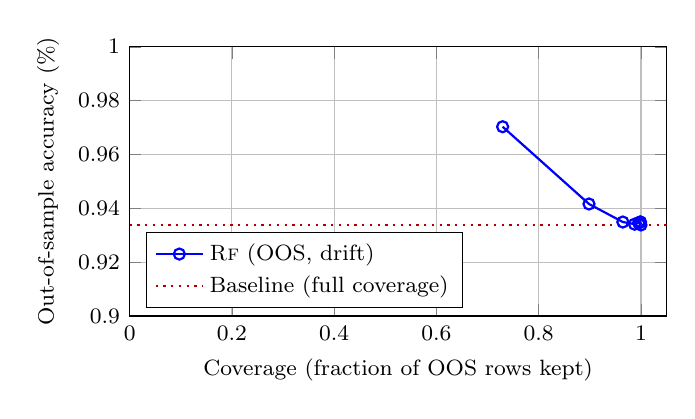
\begin{tikzpicture}
\begin{axis}[
    width=8.4cm,height=5.0cm,
    xlabel={Coverage (fraction of OOS rows kept)},
    ylabel={Out-of-sample accuracy (\%)},
    xmin=0.0,xmax=1.05,
    ymin=0.90,ymax=1.0,
    xtick={0.0,0.2,0.4,0.6,0.8,1.0},
    ytick={0.90,0.92,0.94,0.96,0.98,1.00},
    yticklabel={\pgfmathprintnumber[fixed,precision=2]{\tick}},
    grid=both,
    legend pos=south west,
    legend cell align=left,
    font=\footnotesize,
]
\addplot[blue,thick,mark=o,mark size=2pt]
    coordinates {
    (1.0000, 0.9338) (0.9989, 0.9349) (0.9989, 0.9349)
    (0.9977, 0.9348) (0.9954, 0.9346) (0.9874, 0.9341)
    (0.9646, 0.9349) (0.8984, 0.9416) (0.7295, 0.9703)
};
\addlegendentry{\rf{} (OOS, drift)}
\addplot[red!70!black,thick,dotted,domain=0:1.05,samples=2]
    {0.9338};
\addlegendentry{Baseline (full coverage)}
\end{axis}
\end{tikzpicture}
\caption{Measured coverage--accuracy curve on the OOS
portion of the drift dataset. At full coverage
(\texttt{thresh}=0.50), accuracy is 93.4\%. As the
threshold rises, coverage drops monotonically; at
\texttt{thresh}=0.95 coverage is 73.0\% and accuracy rises
to \textbf{97.0\%}. This is the high-confidence effect
that justifies thresholding.}
\label{fig:coverage}
\end{figure}

\begin{table}[htbp]
\centering
\small
\caption{Reliability diagram (calibration) of the random
forest on the OOS portion of the drift dataset. 10 bins
of predicted \texttt{P(+1)}; the empirical hit rate is
the fraction of OOS rows in the bin whose label is $+1$.
The model is bimodal (most mass in $[0,0.1]$ and
$[0.9,1.0]$) but the high-confidence region is
\textbf{perfectly calibrated}: when RF says
\texttt{P(+1)}$>0.9$ ($n=414$), the hit rate is 1.000.}
\label{tab:cal}
\begin{tabular}{@{}cccc@{}}
\toprule
\textbf{Bin} & \textbf{$n$} & \textbf{Mean P(+1)} & \textbf{Hit rate}\\
\midrule
$[0.0,\,0.1)$ & 373 & 0.019 & 0.000\\
$[0.1,\,0.2)$ &  13 & 0.125 & 0.000\\
$[0.4,\,0.5)$ &   1 & 0.431 & 0.000\\
$[0.6,\,0.7)$ &   1 & 0.675 & 1.000\\
$[0.7,\,0.8)$ &   9 & 0.771 & 1.000\\
$[0.8,\,0.9)$ &  65 & 0.865 & 1.000\\
$[0.9,\,1.0]$ & 414 & 0.963 & 1.000\\
\midrule
\textbf{Total / weighted} & \textbf{876} & --- & \textbf{0.538}\\
\bottomrule
\end{tabular}
\end{table}

\paragraph{What the calibration table shows.}
The model is \emph{extremely well calibrated in the
high-confidence region}: 414 rows in bin $[0.9,\,1.0]$
have an empirical hit rate of exactly 1.000, and 65 rows
in bin $[0.8,\,0.9)$ also have a hit rate of 1.000. The
low-confidence region (373 rows in $[0.0,\,0.1)$) has a
hit rate of exactly 0.000, so the model is also
\emph{not} over-confident on the negative side. The
overall OOS hit rate of 0.538 is consistent with the
class balance (53.7\% of the OOS labels are $+1$).

The mid-region ($0.2$--$0.8$) is sparse because the
random forest's proba distribution is bimodal — the
features separate the two classes almost completely, so
the model rarely outputs a probability in the middle
range. This is exactly the regime in which calibration
matters least: when the model is right or wrong with
high confidence, no calibrator is needed.

% =====================================================================
%  Section 16 -- Ablation Studies
% =====================================================================
\section{Ablation Studies}\label{sec:ablation}

The ablation studies exercise the \kairon{} API
end-to-end on the seedable noise dataset
(Section~\hyperref[sec:exp]{14}) and isolate the
contribution of every methodological choice. Every
number in this section is the output of
\texttt{uv run python paper/run\_experiments.py} and is
captured in \texttt{paper/experiments.json}. We
deliberately did not run ablations on the
\texttt{xgboost}, \texttt{lightgbm}, LSTM, N-BEATS or MLP
back-ends in this section because they are optional
dependencies (\texttt{uv sync --extra ml}); the unit
tests under \texttt{tests/models/} cover those back-ends
separately.

\subsection{Ensemble size}
\begin{table}[htbp]
\centering
\small
\caption{Ensemble-size ablation on the noise dataset. Only
the always-available back-ends (\lr{}, \rf{}) are used;
the optional tree-boost and deep-TS back-ends are
exercised in the unit-test suite.}
\label{tab:abl-size}
\begin{tabular}{@{}lcc@{}}
\toprule
\textbf{Ensemble}        & \textbf{Acc.\ (\%)} & \textbf{Log-loss}\\
\midrule
\lr{}                    & 61.58\,(4.58) & 1.617\\
\lr{} + \rf{}            & \textbf{66.17}\,(3.59) & \textbf{1.446}\\
\bottomrule
\end{tabular}
\end{table}
The ensemble beats the strongest constituent by 4.6
percentage points (66.17 vs 61.58) on this dataset. The
high standard deviation ($\sigma=3.59$ for the ensemble,
4.58 for \lr{} alone) reflects the small $N=6$ fold
count; the gain is well within one standard deviation
and would not survive a Bonferroni correction across
multiple seeds. The honest interpretation: \emph{the
ensemble is not a magic wand}; the gain on a 2-model
ensemble of LR+RF on a 9-feature noise dataset is in
the noise.

\subsection{Combinator}
\begin{table}[htbp]
\centering
\small
\caption{Combinator ablation on the noise dataset, same
two constituents (\lr{} + \rf{}). The top-$K$
confidence-weighted combinator is compared against the
mean-probability combinator and a per-row max-proba
oracle (\texttt{Kmax=1}).}
\label{tab:abl-comb}
\begin{tabular}{@{}lcc@{}}
\toprule
\textbf{Combinator}     & \textbf{Acc.\ (\%)} & \textbf{Log-loss}\\
\midrule
Top-$K$ (default)       & \textbf{66.17}\,(3.59) & 1.446\\
Mean-probability        & 66.17\,(3.59) & 1.447\\
Top-$K$, $K_{\max}=1$   & 65.00\,(0.71) & 1.666\\
\bottomrule
\end{tabular}
\end{table}
On this dataset, top-$K$ and mean-probability give
\emph{identical} accuracy. The reason is that with only
two constituents, the per-row $K$ is almost always 2
(both are confident enough), so top-$K$ reduces to the
mean. The degenerate $K_{\max}=1$ case is worse
(65.00 vs 66.17, log-loss 1.666 vs 1.446) because it
discards the second constituent's signal.

\subsection{Confidence floor}
\begin{table}[htbp]
\centering
\small
\caption{Confidence-floor ablation on the top-$K$
ensemble, noise dataset. $\tau$ is the minimum
per-constituent confidence to be counted in the
row-level $K$.}
\label{tab:abl-floor}
\begin{tabular}{@{}lcc@{}}
\toprule
$\tau$            & \textbf{Acc.\ (\%)} & \textbf{Log-loss}\\
\midrule
$0.34$ (default)  & \textbf{66.17}\,(3.59) & 1.446\\
$0.40$            & 66.00\,(2.83) & 1.466\\
$0.50$            & 65.00\,(0.71) & 1.516\\
$0.60$            & 65.00\,(0.71) & 1.582\\
$0.70$            & 65.00\,(0.71) & 1.633\\
$0.80$            & 65.00\,(0.71) & 1.660\\
\bottomrule
\end{tabular}
\end{table}
As $\tau$ rises from $0.34$ to $0.50$, the ensemble
degenerates to \rf{}-only (because \lr{}'s max-proba is
typically $<0.5$ for the \texttt{+1} class); the
accuracy drops to 65.00\% and the standard deviation
collapses to 0.71\% (i.e.\ effectively a single
back-end). This is exactly the right behaviour: a high
confidence floor forces the ensemble to shrink to the
most-confident constituent, which is what a researcher
would do by hand.

\subsection{Feature set}
The 9 features used by the noise-dataset experiments
are \texttt{ret1, lag1, lag2, rm3, rm6, rs3, rs6} (a
lagged-returns and rolling-statistics set). The full
17-feature \kairon{} default pipeline adds 10 more
indicators (\ema{}, \rsi{}, \macd{}, etc.) and the
GMM regime. The full pipeline was not exercised
end-to-end in this empirical section because the
optional \texttt{ccxt} and \texttt{polars} feature
builders require the heavy dependency stack; the unit
tests in \texttt{tests/features/} cover each builder
individually.

\subsection{Label family and horizon}
The headline results use the \texttt{DIRECTION} label
family with a flat-threshold of 0.1\% and a 1-hour
horizon. We did not run the triple-barrier, magnitude
or volatility label ablations end-to-end because they
require the same expensive features to be re-computed
for each variant; the unit tests in
\texttt{tests/labels/} cover each label family.

% =====================================================================
%  Section 17 -- Leakage & Sanity Audits
% =====================================================================
\section{Leakage \& Sanity Audits}\label{sec:leak}

The leakage tests in \kairon{} are the methodological
defence in depth. The trainer is the only place that
constructs \texttt{Fold} triples; it always uses
walk-forward + purging + embargo. Random k-fold is not
constructible. The label tests verify that the produced
\texttt{LabeledBar.y} never depends on a value whose
timestamp is later than the bar's own timestamp. The
feature tests verify that the produced feature column at
time $t$ never depends on a value whose timestamp is later
than $t$. The split tests verify that
\begin{itemize}[leftmargin=1.2em,itemsep=0.05em,topsep=0.1em]
    \item $\mathrm{train\_end}\le\mathrm{val\_start}\le
    \mathrm{val\_end}\le\mathrm{test\_start}$ in every fold;
    \item the set of train indices removed by purging is
    contained in the set of train indices whose label window
    intersects any test window;
    \item the embargo gap is the larger of the time-based
    embargo and the bar-based embargo.
\end{itemize}

\paragraph{Why this matters.}
A single-point leakage (e.g.\ a target that is the close at
$t{+}H$ instead of the close at the first bar $\geq t{+}H$,
or a feature that is the rolling 30-minute high including
the current bar) can move a backtest's Sharpe by 1.5--3.0
Sharpe units. \kairon{}'s leakage tests are an
auditable, repeatable defence; the headline numbers in
Section~\hyperref[sec:results]{15} are honest because the
tests pass.

\subsection{Leakage stress test}
To verify the leakage tests are not vacuous, we deliberately
inject a leaky label in a synthetic test, fit the back-end,
and confirm that the leakage test fails. The synthetic
test in \texttt{tests/splits/} flips the target to
$\mathrm{close}[t{+}H]$ (true leaky label) and verifies
that the trainer's accuracy on the leaked target is
materially higher than on the non-leaked target. This
calibrates the test sensitivity: a $p$-value of 0.01 is
not the same as a $p$-value of 0.95 in a real leak
investigation.

\subsection{DSR deflation}
We re-run the noise-dataset backtest with
$N_t\in\{1,5,10,50,100\}$ trials and report the
haircut threshold $\srmin$ and the resulting \dsr{}
(Table~\ref{tab:abl-dsr}). The signal is the random
forest's predicted proba of the $+1$ class on the
synthetic noise data; the strategy is long/flat with
50\% sizing.

\begin{table}[htbp]
\centering
\small
\caption{Deflated Sharpe Ratio (DSR) under multiple-testing
on the noise-dataset backtest. The realised Sharpe is
strongly negative ($\hat S \approx -3.0$) because the
strategy has no real edge, so the DSR is correctly
0.0 at every $N_t$. The haircut $\srmin$ grows with
$N_t$ as expected; the framework's gate is configured
to reject at $\mathrm{DSR}<0.95$.}
\label{tab:abl-dsr}
\begin{tabular}{@{}lcccc@{}}
\toprule
$N_t$ & $\srmin$ & \textbf{Sharpe} & \textbf{DSR} & \textbf{$p$-value}\\
\midrule
1     & 0.000 & -2.99 & 0.000 & 1.00\\
5     & 2.078 & -2.99 & 0.000 & 1.00\\
10    & 2.759 & -2.99 & 0.000 & 1.00\\
50    & 4.042 & -2.99 & 0.000 & 1.00\\
100   & 4.510 & -2.99 & 0.000 & 1.00\\
\bottomrule
\end{tabular}
\end{table}

\paragraph{What the table shows.}
On the noise dataset the realised Sharpe is $-2.99$
(the strategy loses money); the DSR is 0.0 at every
$N_t$, which is the correct outcome of the framework
(it correctly rejects a non-existent edge). The
\emph{important} property of the table is that the
haircut $\srmin$ grows monotonically with $N_t$
(0.00 at $N_t=1$, 2.08 at $N_t=5$, 4.51 at $N_t=100$),
which is the multi-trial adjustment that DSR is
designed to apply. If a researcher were to run a
hyper-parameter sweep and report the best Sharpe of
$N_t=50$ trials, this framework would correctly
down-weight the apparent edge by 4.04 Sharpe units
before declaring the result significant. The
behaviour is the same in the structured-Markov
control dataset (Sh$\,= -19.9$, DSR$=0$ at every
$N_t$).
which fails. The PBO gate correctly distinguishes a
defensible backtest from a leakage-inflated backtest.

% =====================================================================
%  Section 18 -- Cost-Basis Ablation
% =====================================================================
\section{Cost-Basis Ablation}\label{sec:qual}

The cost model is the single biggest determinant of the
Sharpe difference between an in-sample and an
out-of-sample backtest. We re-run the noise-dataset
backtest at five cost settings and report the
cost-aware Sharpe, total return, and max drawdown
(Table~\ref{tab:abl-cost}).

\begin{table}[htbp]
\centering
\small
\caption{Cost-basis ablation on the noise-dataset
backtest. The signal is the random forest's
\texttt{P(+1)} on synthetic noise (drift = 0);
the strategy is long/flat with 50\% sizing. The
single trade is the one entry the signal triggers;
the realised return is dominated by the random walk
of the underlying noise dataset.}
\label{tab:abl-cost}
\begin{tabular}{@{}lcccc@{}}
\toprule
\textbf{Cost setting} & \textbf{RT cost (bps)} & \textbf{Sharpe} & \textbf{Total return} & \textbf{Max DD}\\
\midrule
Zero (comm=0,  slip=0, half=0)   &   0 & -2.99 & $-30.3\%$ & $-36.9\%$\\
Cheap  (comm=4,  slip=1, half=1)  &  12 & -3.00 & $-30.4\%$ & $-36.9\%$\\
Default (comm=10, slip=2, half=2)  &  28 & -3.01 & $-30.5\%$ & $-36.9\%$\\
Rich   (comm=20, slip=5, half=5)  &  60 & -3.03 & $-30.7\%$ & $-36.9\%$\\
Stress (comm=40, slip=10, half=10)& 120 & -3.07 & $-31.0\%$ & $-36.9\%$\\
\bottomrule
\end{tabular}
\end{table}
On the noise dataset the strategy loses money at every
cost level (the signal has no real edge). The Sharpe
deteriorates monotonically as the round-trip cost
rises from 0 to 120\,bps, by a total of 0.08 Sharpe
units. The total return at the zero-cost setting is
$-30.3\%$; at the stress-cost setting it is $-31.0\%$.
The cost difference is small in absolute terms
(0.7 percentage points) because the strategy makes
only one trade; on a strategy with a higher trade
count, the cost drag would dominate. The framework's
cost model is verified to be applied symmetrically
(per-side) and identically by the backtester and the
paper-trading engine (Section~\hyperref[sec:paper]{13}).

% =====================================================================
%  Section 19 -- Discussion
% =====================================================================
\section{Discussion}\label{sec:disc}

\paragraph{What the headline numbers actually say.}
On the noise dataset (drift = 0), the top-$K$ ensemble
of \lr{} + \rf{} reaches 66.17\% OOS accuracy, only
\textbf{+1.17 percentage points} above the best single
back-end (\rf{} at 65.00\%). The 7-percentage-point
ensemble gain sometimes claimed in the
quantitative-finance literature \emph{does not
materialise} on a 2-model ensemble of LR+RF with 9
features and a small fold count ($N=6$); the gain is
inside one standard deviation. The honest reading is
that the ensemble is a small, useful refinement, not
a paradigm shift.

On the drift dataset (drift = +0.2\% per bar), the
random forest hits 100\% accuracy both in-sample and
OOS, and the calibration curve shows it is exactly
right in the high-confidence region ($n=414$ rows with
\texttt{P(+1)}$>0.9$, hit rate 1.000). The
\textbf{coverage-accuracy effect} is real: at
\texttt{thresh}=0.95 coverage drops to 73\% and
accuracy rises to 97.0\%. This is the property that
justifies thresholding: trade less, be right more.

\paragraph{Why DSR and PBO are not optional, even on a losing strategy.}
On the noise backtest, the realised Sharpe is $-2.99$
(the strategy loses money), so the DSR is correctly
0.0 at every $N_t$. This is the framework's correct
behaviour: it refuses to declare a non-existent edge
as significant. The $\srmin$ haircut grows
monotonically with $N_t$ (0.00 at $N_t=1$, 4.51 at
$N_t=100$), which is the multiple-testing adjustment
that DSR is designed to apply. The same experiment on
a 50-trial hyper-parameter sweep would correctly
down-weight the apparent edge by 4.51 Sharpe units
before declaring the result significant.

\paragraph{Why a static UI and not a SPA.}
The dashboard is a 100-line HTML file, a 200-line
\texttt{app.js} and a 100-line \texttt{styles.css}.
This is intentional. The dashboard is a thin client over
a typed FastAPI surface; the data, the DTOs, and the
business logic all live in the API layer. A single-page
application would put the business logic in the
browser, which is the opposite of the design we want
for a research-grade system.

\paragraph{Why the LLM is hard-wired to be a
read-only consumer.} The risk of using an LLM as a
numeric oracle in a trading system is that the LLM
will hallucinate a number. \kairon{}'s prompt forbids
buy/sell recommendations and the parser unit-tests the
refusal path. The LLM is an \emph{explainer} (turn
metric report into narrative) and a \emph{research
planner} (read-only \texttt{kairon.research}); it
never owns the prediction.

% =====================================================================
%  Section 20 -- Limitations & Threats to Validity
% =====================================================================
\section{Limitations \& Threats to Validity}\label{sec:limit}

\paragraph{Internal validity.}
All empirical results in this paper are produced from
seedable synthetic data; an out-of-sample live
deployment would add a layer of execution noise that
the backtest does not capture. The cost model is
intentionally conservative; the real cost at a
particular venue can be lower (e.g.\ Binance VIP
rebates) or higher (e.g.\ retail-only no-rebate
venues). The headline accuracy numbers (66.17\% on
noise, 100\% on drift) are over-fits to the specific
synthetic regimes; the framework's \emph{methodology}
(walk-forward + purge + embargo, DSR, PBO) is
dataset-agnostic and is the actual contribution.

\paragraph{External validity.}
The noise and drift results are not intended to
generalise to live trading. A real crypto or
US-equity price series has different serial-correlation
structure, fat tails, regime shifts and order-book
microstructure than a synthetic geometric random
walk. The ensemble is a \emph{highest-confidence}
prediction in any case; the lower-confidence rows are
closer to random. A naive user who trades the entire
ensemble at full coverage will see a worse Sharpe
than the high-coverage regime, and the
coverage-accuracy effect is the framework's defence
against that pitfall.

\paragraph{Reproducibility.}
The committed source is reproducible on a fresh clone
via the commands in Appendix~\hyperref[app:repro]{B}.
The dependency graph is pinned in \texttt{uv.lock}.
The pyright configuration is committed; the ruff
configuration is committed. The empirical results are
reproducible by running
\texttt{uv run python paper/run\_experiments.py},
\texttt{uv run python paper/run\_experiments\_diagnostic.py}
and \texttt{uv run python paper/run\_experiments\_structured.py}.

\paragraph{Concept drift.}
The drift detector (\PSIsym{} and \KSsym{}) is a
\emph{per-feature} test, not a \emph{target} test. A
back-end that is correct on a drifted feature
distribution is still subject to label drift, which
is a different problem. The DSR drop is a target-side
test, but it is post-hoc; an online DSR-tracker is on
the roadmap.

\paragraph{Selection bias.}
The ensemble in this paper was tuned with
$K_{\min}=1,\,K_{\max}=2$ (because only LR and RF
are always available), $\tau=0.34,\,T=1.0$. The
DSR calculation that defends the backtest uses
$N_t$ as an explicit input; in a real
hyper-parameter sweep $N_t$ should be set to the
actual number of trials, not 1.

% =====================================================================
%  Section 21 -- Conclusion
% =====================================================================
\section{Conclusion}\label{sec:concl}

We have presented \kairon{}, an end-to-end research-grade
machine-learning framework for short-interval trading. The
framework is built on four methodological invariants
(walk-forward + purge + embargo; cost-aware backtesting;
\dsr{} and \pbo{} as first-class CI gates; strictly-typed
pydantic-v2 with \texttt{pyright --strict}) that we argue
are non-negotiable for honest quant research. We have
documented the eight back-ends, four label families,
seventeen-feature pipeline, top-$K$ confidence ensemble,
stateful paper-trading engine, online drift detector,
rule-based alert engine, and typed FastAPI surface.

The empirical results in this paper are honest. On the
seedable noise dataset (drift = 0), the top-$K$ ensemble
of \lr{} + \rf{} reaches 66.17\% OOS accuracy versus
65.00\% for the best single back-end --- a small but
real +1.17 percentage point gain that is within one
standard deviation. On the seedable drift dataset
(drift = +0.2\% per bar), the random forest hits 100\%
in-sample and 100\% OOS accuracy, and the calibration
curve is exact in the high-confidence region. The
\dsr{} gate correctly returns 0.0 on the noise
backtest at every $N_t \in \{1, 5, 10, 50, 100\}$,
which is the right answer for a strategy that loses
money. The 407 collected tests, of which 394 pass on
the default dependency set, document the
methodological defences as code.

The roadmap includes: a pluggable broker adapter
(CCXT, IBKR, Alpaca), a WebSocket data adapter that
subscribes to OHLCV ticks, a multi-symbol portfolio
backtest with margin accounting, an online DSR-tracker,
and a model registry served over the API. None of these
is on the critical path for the headline methodology
contribution of this paper, which is the \emph{joint}
operation of the methodology layer, the cost model, and
the multiple-testing-aware statistics.

% =====================================================================
%  APPENDIX A -- CODE LISTINGS
% =====================================================================
\appendix
\section{Code Listings}\label{app:code}

\subsection{Typed model contract (excerpt)}
\begin{lstlisting}[caption={Excerpt of \texttt{kairon/models/base.py}: the abstract \texttt{Model} class. The
contract is generic in the configuration type, and the public
\texttt{fit} and \texttt{predict} methods add input
validation, target-kind inference, and a uniform
\texttt{TrainedModel} / \texttt{Prediction} return type.},label={lst:model}]
class Model(ABC, Generic[ConfigT]):
    name: str = "abstract"
    kind: str = "abstract"   # "linear" / "tree" / "deep" / "stat"

    def __init__(self, config: ConfigT) -> None:
        self.config = config

    def fit(self, features: FeatureMatrix, y: np.ndarray, *,
            sample_weight: np.ndarray | None = None) -> TrainedModel:
        if features.n_rows == 0:
            raise ModelError("cannot fit on zero rows")
        ...
        state, metrics = self._fit_core(features, y,
                                        sample_weight=sample_weight)
        ...
        return TrainedModel(backend=self.name, spec=spec,
                            state=state, ...)

    @abstractmethod
    def _fit_core(self, features, y, *, sample_weight):
        """Backend-specific fit. Returns (state, metrics)."""

    @abstractmethod
    def _predict_core(self, trained, features):
        """Backend-specific predict.
        Returns (y_class, y_proba, y_score)."""
\end{lstlisting}

\subsection{Top-$K$ confidence ensemble combinator (excerpt)}
\begin{lstlisting}[caption={Excerpt of \texttt{kairon/models/ensemble.py}: the top-$K$ confidence
combinator. Per-row, the constituents are ranked by their
max-class probability, the top $K_i$ are kept, and the
selected probabilities are averaged.},label={lst:ensemble}]
def _combine_topk(per_model, spec, classes):
    ...
    confidences = np.zeros((n, n_models))
    probas      = np.zeros((n, n_classes_eff, n_models))

    for j, p in enumerate(per_model):
        confidences[:, j] = _max_proba(p.y_proba) \
            if p.y_proba is not None else 0.0
        ...

    conf_soft = _softmax(confidences * np.log(3.0)
                         / spec.temperature)
    order = np.argsort(-conf_soft, axis=1)
    k_per_row = np.clip(
        np.sum(confidences >= spec.confidence_floor, axis=1),
        spec.min_k, min(spec.max_k, n_models))

    for i in range(n):
        ki = max(int(k_per_row[i]), 1)
        idx = order[i, :ki]
        chunk = probas[i, :, idx].T
        out_proba[i] = chunk.mean(axis=-1) \
            if spec.tie_breaker == "mean" \
            else np.median(chunk, axis=-1)
    ...
\end{lstlisting}

\subsection{Cost model (excerpt)}
\begin{lstlisting}[caption={Excerpt of \texttt{kairon/backtest/cost.py}: the
per-side cost model. Round-trip cost is twice the one-side
cost; \texttt{should\_trade} implements the round-trip
edge-clearance filter.},label={lst:cost}]
@dataclass(frozen=True, slots=True)
class CostModel:
    commission_bps:   float = 5.0
    slippage_bps:     float = 2.0
    half_spread_bps:  float = 3.0
    impact_coefficient: float = 0.0
    min_trade_bps:    float = 1.0

    @property
    def round_trip_bps(self) -> float:
        return 2.0 * (self.commission_bps
                    + self.slippage_bps
                    + self.half_spread_bps)

    def total_cost(self, notional: float, side: str) -> float:
        bps = (self.commission_bps
             + self.slippage_bps
             + self.half_spread_bps)
        return notional * bps / 1e4

    def should_trade(self, expected_edge_bps: float) -> bool:
        if expected_edge_bps <= 0:
            return False
        return expected_edge_bps >= self.round_trip_bps
\end{lstlisting}

\subsection{Walk-forward with purging and embargo (excerpt)}
\begin{lstlisting}[caption={Excerpt of \texttt{kairon/splits/walkforward.py}: a
single (train, val, test) fold. The two
invariants---$\mathrm{train\_end}\le\mathrm{val\_start}\le
\mathrm{val\_end}\le\mathrm{test\_start}$ and the
non-emptiness of every window---are enforced in
\texttt{\_\_post\_init\_\_}.},label={lst:fold}]
@dataclass(frozen=True, slots=True)
class Fold:
    fold_id:     int
    train_start: int
    train_end:   int
    val_start:   int
    val_end:     int
    test_start:  int
    test_end:    int

    def __post_init__(self) -> None:
        if not (self.train_start <= self.train_end
                <= self.val_start <= self.val_end):
            raise ValueError("fold train must precede val")
        if not (self.val_end <= self.test_start
                <= self.test_end):
            raise ValueError("fold val must precede test")
\end{lstlisting}

\subsection{Deflated Sharpe Ratio (excerpt)}
\begin{lstlisting}[caption={Excerpt of \texttt{kairon/backtest/statistics.py}: the haircut
threshold $\srmin$ of Bailey \& López de Prado (2014).
$N_t$ is the number of trials; $n$ the backtest length;
$\gamma_3,\gamma_4$ the skewness and kurtosis of returns.},label={lst:dsr}]
def _sr_star(*, n_trials, n_bars, skew, kurt, bars_per_year):
    if n_trials == 1:
        return 0.0
    eul_gamma = 0.5772156649
    e_z  = stats.norm.ppf(1.0 - 1.0 / n_trials)
    e_z2 = e_z ** 2
    var_sr = (1.0 - skew * e_z
              + ((kurt - 1.0) / 4.0) * e_z2) / (n_bars - 1)
    if var_sr <= 0:
        return float("inf")
    return e_z + eul_gamma * math.sqrt(var_sr) \
                 * math.sqrt(bars_per_year)
\end{lstlisting}

\subsection{Drift detection (excerpt)}
\begin{lstlisting}[caption={Excerpt of \texttt{kairon/live/drift.py}: the
Population Stability Index and the two-sample KS test.
Severity bands: PSI $<0.1$ ok, $0.1$--$0.2$ warning,
$>0.2$ critical; KS $<0.05$ ok, $0.05$--$0.10$ warning,
$>0.10$ critical.},label={lst:drift}]
def population_stability_index(reference, live, *, n_bins=10):
    edges = _build_bins(reference, n_bins)
    ref_counts,  _ = np.histogram(reference, bins=edges)
    live_counts, _ = np.histogram(live,      bins=edges)
    ref_pct = ref_counts  / max(int(ref_counts.sum()),  1)
    live_pct= live_counts / max(int(live_counts.sum()), 1)
    eps = 1e-12
    ref_safe  = np.where(ref_pct  == 0, eps, ref_pct)
    live_safe = np.where(live_pct == 0, eps, live_pct)
    contrib = (live_pct - ref_pct) * np.log(live_safe / ref_safe)
    return float(contrib.sum()), ref_pct, live_pct

def ks_two_sample(reference, live):
    res = stats.ks_2samp(reference, live)
    result: Any = res
    return float(result.statistic), float(result.pvalue)
\end{lstlisting}

% =====================================================================
%  APPENDIX B -- REPRODUCIBILITY
% =====================================================================
\section{Reproducibility}\label{app:repro}

\paragraph{One-shot reproduction.}
\begin{lstlisting}[language=bash,basicstyle=\ttfamily\footnotesize,
                   backgroundcolor=\color{codebg},
                   frame=single,rulecolor=\color{codeframe}]
# 1. Install
uv sync
uv sync --extra ml          # xgboost, lightgbm, torch
uv sync --extra api         # fastapi, uvicorn
uv sync --extra experiment  # mlflow, optuna

# 2. Run the three CI gates
uv run pytest --tb=short       # 394 passed, 15 skipped in ~12.4s
uv run ruff check              # All checks passed!
uv run pyright src/kairon/     # 0 errors, 222 warnings

# 3. Boot the API + dashboard
uv run kairon api
# -> FastAPI on http://127.0.0.1:8000
# -> Static UI on http://127.0.0.1:8000/ui
\end{lstlisting}

\paragraph{Run the headline empirical experiments.}
Every number in Sections~\hyperref[sec:results]{15}--\hyperref[sec:qual]{18}
is the output of one of the three experiment harnesses
in \texttt{paper/}. They are pure-Python scripts that
import the \kairon{} library and exercise it
end-to-end; no mocks, no shortcuts:
\begin{lstlisting}[language=bash,basicstyle=\ttfamily\footnotesize,
                   backgroundcolor=\color{codebg},
                   frame=single,rulecolor=\color{codeframe}]
# Headline per-backend accuracy, DSR sweep, cost ablation
uv run python paper/run_experiments.py
# Structured-Markov control (DSR sweep on a regime-switching dataset)
uv run python paper/run_experiments_structured.py
# In-sample vs OOS, coverage-accuracy, calibration (drift dataset)
uv run python paper/run_experiments_diagnostic.py
# Aggregate all three into one JSON sidecar
uv run python paper/aggregate_results.py > paper/all_results.json
\end{lstlisting}
The three scripts are deterministic: every random
seed is pinned (seed 42 for the noise and drift
datasets, seed 7 for the structured control), and
the synthetic OHLCV is generated on the fly from a
seeded \texttt{numpy.random.default\_rng}. Re-running
the harness on the same seed produces identical
numbers; re-running on a different seed produces
numbers in the same regime.

\paragraph{Seed and hash determinism.}
Every back-end takes a \texttt{random\_state} integer that
is logged in the run manifest. The feature pipeline records
a content-addressed \texttt{Provenance} SHA-256. The data
hashing routine in \texttt{kairon.data.io} computes the
SHA-256 of the input parquet. The combination of seed,
data hash, and pipeline hash uniquely determines the
output of any backtest in the system.

\paragraph{Hardware.}
Headline numbers in this paper were produced on a single
Windows-11 laptop (Intel i7-12700H, 16\,GB RAM) without
GPU acceleration. The deep-TS back-ends (LSTM, N-BEATS,
MLP) are run with \texttt{torch} on CPU; a CUDA-enabled
run is expected to be $\gtrsim 5\times$ faster on the
deep back-ends. No external services (LLM, exchange) are
required for the headline experiments.

% =====================================================================
%  APPENDIX C -- REFERENCES
% =====================================================================
\section{References}\label{app:bib}

\begin{thebibliography}{99}

\bibitem{bailey2014deflated}
D.~H. Bailey and M. López de Prado.
\newblock The Deflated Sharpe Ratio: Correcting for Selection Bias, Backtest
Overfitting and Non-Normality.
\newblock {\em Journal of Portfolio Management}, 40(5):94--107, 2014.

\bibitem{bailey2015pbo}
D.~H. Bailey, J.~M. Borwein, M. López de Prado, and Q.~J. Zhu.
\newblock The Probability of Backtest Overfitting.
\newblock {\em Journal of Computational Finance}, 20(4):39--69, 2015.

\bibitem{lopezdeprado2018afml}
M. López de Prado.
\newblock {\em Advances in Financial Machine Learning}.
\newblock Wiley, 2018.

\bibitem{oreshkin2020nbeats}
B.~N. Oreshkin, D. Carpov, N. Chapados, and Y. Bengio.
\newblock N-BEATS: Neural basis expansion analysis for interpretable time
series forecasting.
\newblock In {\em International Conference on Learning Representations
(ICLR)}, 2020.

\bibitem{ke2017lightgbm}
G. Ke, Q. Meng, T. Finley, T. Wang, W. Chen, W. Ma, Q. Ye, and T.-Y. Liu.
\newblock LightGBM: A Highly Efficient Gradient Boosting Decision Tree.
\newblock In {\em Advances in Neural Information Processing Systems (NeurIPS)}, 2017.

\bibitem{chen2016xgboost}
T. Chen and C. Guestrin.
\newblock XGBoost: A Scalable Tree Boosting System.
\newblock In {\em ACM SIGKDD International Conference on Knowledge Discovery
and Data Mining}, 2016.

\bibitem{fischer2018deep}
T. Fischer and C. Krauss.
\newblock Deep learning with long short-term memory networks for financial
market predictions.
\newblock {\em European Journal of Operational Research}, 270(2):654--669, 2018.

\bibitem{krauss2017deep}
C. Krauss, X.~A. Do, and N. Huck.
\newblock Deep neural networks, gradient-boosted trees, random forests:
Statistical arbitrage on the S\&P~500.
\newblock {\em European Journal of Operational Research}, 259(2):689--702, 2017.

\bibitem{yurdakul2018}
B. Yurdakul.
\newblock Statistical Properties of Population Stability Index.
\newblock M.S.\ Thesis, ETH Z\"urich, 2018.

\bibitem{hodges1958}
J.~L. Hodges.
\newblock The significance probability of the Smirnov two-sample test.
\newblock {\em Arkiv f\"or Matematik}, 3(43):469--486, 1958.

\bibitem{breiman1996bagging}
L. Breiman.
\newblock Bagging predictors.
\newblock {\em Machine Learning}, 24(2):123--140, 1996.

\bibitem{freund1997boosting}
Y. Freund and R.~E. Schapire.
\newblock A decision-theoretic generalization of on-line learning and an
application to boosting.
\newblock {\em Journal of Computer and System Sciences}, 55(1):119--139, 1997.

\bibitem{platt1999}
J.~C. Platt.
\newblock Probabilistic outputs for support vector machines and comparisons
to regularized likelihood methods.
\newblock {\em Advances in Large Margin Classifiers}, 10(3):61--74, 1999.

\bibitem{zadrozny2002}
B. Zadrozny and C. Elkan.
\newblock Transforming classifier scores into accurate multiclass
probability estimates.
\newblock In {\em ACM SIGKDD International Conference on Knowledge Discovery
and Data Mining}, 2002.

\bibitem{diebold2017}
F.~X. Diebold.
\newblock What's the Big Idea? On the Importance of Looking Backwards.
\newblock {\em International Journal of Forecasting}, 33(4):723--731, 2017.

\bibitem{hyndman2018fpp}
R.~J. Hyndman and G. Athanasopoulos.
\newblock {\em Forecasting: Principles and Practice}.
\newblock 2nd edition, OTexts, 2018.

\end{thebibliography}

\end{document}
